\chapter{Test Amplification For Artificial Behavioral Changes Detection}
\label{chap:test-improvement}

\begin{chaptersummary}
	In this chapter, I detail a first evaluation of \dspot. 
	This evaluation is based on the mutation score as test-criterion.
	Mutation score measures the test suite's ability to detect artificial behavioral changes.
	I performed this evaluation 40 test classes from 10 projects from \gh and show that \dspot improve 26 of them.
	I also confronted \dspot's output to the real by proposing the amplified test methods to the developers through pull-requests.
	These pull requests showed developers' interest in the result of \dspot.
	
	To sum up, the contributions of this chapter are:
	\begin{itemize}
		\item the design and execution of an experiment to assess the relevance of \dspot, based on feedback from the developers of mature projects;
		\item a large scale quantitative study of the improvement of 40 real-world test classes taken from 10 mature open-source Java projects.	
		\item fully open-science code and data: both \dspot\footnote{\url{https://github.com/STAMP-project/dspot/}} and our experimental data are made publicly available for future research\footnote{\url{https://github.com/STAMP-project/dspot-experiments/}}
	\end{itemize}
	Note that this chapter has been published~\cite{Danglot2019}.
\end{chaptersummary}

\minitoc

\graphicspath{{.}{chapitres/test-improvement/}}

% ---------------------------------------------------------------------------------------
% INTRODUCTION
% ---------------------------------------------------------------------------------------
\section{Introduction}
\label{sec:test-improvement:introduction}

\subsection{Test-criterion: \ms}
\label{subsec:test-improvement:introduction:test-criterion}

% MS
This chapter relates the first study of the \dspot's effectiveness.
To do this evaluation, I had to choose the test-criterion to select amplified test methods.
I choose to use \ms.
\ms measures the test suite's ability to detect artificial behavioral changes.
Briefly, \ms is measured as follow:
First, it injects a fault, or an artificial behavioral change, in the source code, \eg changes a $\ge$ by a $>$.
This modified program is called ``mutants''.
It generates different mutants with different artificial behavioral change;
Second, it executes the test suite on the mutant;
Third, it collects the result of the execution.
If no test methods fail, it means that the test suite is not able to detect the fault. 
It is said that the mutant remains alive.
If at least on test method fails, it means that the test suite is able to detect the fault.
It is said that the test suite kills the mutant.
Eventually, to compute the \ms, one must compute the percentage of mutants killed over the mutants generated.
The more mutants the test suite kills, the better is considered the test suite.
\ms aims at emulating faults that a developer could integrate in its code.
If the test suite has a high \ms, the probability that it detect such fault decrease.

\dspot uses \pitest \footnote{latest version released at the time of the experimentation: 1.2.0.\url{https://github.com/hcoles/pitest/releases/tag/1.2.0}} because:
1) it targets Java programs, 
2) it is mature and well-regarded,
3) it has an active community. 

An important feature of \pitest is that if the application code remains unchanged, the generated mutants are always the same.
This property is very interesting for test amplification.
Since \dspot only modifies  test code, this feature allows us to compare the \ms of the original test case against the \ms of the amplified version and even compare the absolute number of mutants killed by both test case variants. 
We will exploit this feature in our evaluation.

By default, \dspot uses all the mutation operators available in \pitest: 
conditionals boundary mutator;
increments mutator;
invert negatives mutator;
math mutator;
negate conditionals mutator;
return values mutator;
void method calls mutator.

\subsection{Mutation score versus coverage}
\label{subsec:test-improvement:introduction:mutation-score-vs-coverage}
In this experimentation, I use the \ms rather than coverage because \ms is consider stronger than coverage.
The purpose of test suites is to check the program's behavior.
In one hand, coverage is only based on the execution of the program and do not require any oracles.
Coverage does not measure the proportion of the behavior tested but only the proportion of code executed.
In the other hand, \ms requires oracles and thus to have a high \ms, the test suite must contains oracles.

The remainder of this chapter is as follows:
\autoref{sec:test-improvement:introduction} introduces this chapter;
\autoref{sec:test-improvement:experiment-protocol} presents the experimental protocol of our study;
\autoref{sec:test-improvement:experiment-results} analyses our empirical results.;
\autoref{sec:test-improvement:threats} discusses the threats to validity;
and \autoref{sec:test-improvement:conclusion} concludes this chapter;

%%%%%%%%%%%%%%%%%%%%%%%%%%%%%%%%%%%%%%%%%%%%%%%%%%%%%%%
% EVALUATION
%%%%%%%%%%%%%%%%%%%%%%%%%%%%%%%%%%%%%%%%%%%%%%%%%%%%%%%
\section{Experimental  Protocol}
\label{sec:test-improvement:experiment-protocol}

\TODO{Automatic test improvement ?????}
Automatic test improvement has been evaluated with respect to evolutionary test inputs \cite{tonella} and new assertions \cite{TaoXie2006}.
However:
1) the two topics have never been studied in conjunction
2) they have never been studied on large modern Java programs
3) most importantly, the quality of improved tests has never been assessed by developers.

I set up a novel experimental protocol that addresses those three points.
First, the experiment is based on \dspot, which combines test input exploration and assertion generation.
Second, the experiment is made on 10 active \gh projects.
Third, I have proposed improved tests to developers under the form of pull-requests.

I answer the following research questions:

\newcommand\rqpullrequest{RQ1\xspace}
\newcommand\rqcandidates{RQ2\xspace}
\newcommand\rqeffectiveness{RQ3\xspace}
\newcommand\rqAmplVersusIAmpl{RQ4\xspace}

\noindent\textbf{\rqpullrequest}: Are the improved test cases produced by \dspot relevant for developers? Are the developers ready to permanently accept the improved test cases into the test repository?\\
\textbf{\rqcandidates}: To what extent are improved test methods considered as focused?\\
\textbf{\rqeffectiveness}: To what extent do the improved test classes increase the \ms of the original,  manually-written, test classes?\\
\textbf{\rqAmplVersusIAmpl}: What is the relative contribution of \Iampl{} and \Aampl{} to the effectiveness of automatic test improvement?\\

\subsection{Dataset}
\label{subsec:test-improvement:experiment-protocol:dataset}

We evaluate \dspot by amplifying test classes of large-scale, notable, open-source projects. The dataset includes projects that fulfill the following criteria:  
1) the project must be written in Java; 
2) the project must have a test suite based on \junit;
3) the project must be compiled and tested with Maven;
4) the project must have an active community as defined by the presence of pull requests on \gh, see \autoref{subsubsec:answer-rqpullrequest}. 

	\begin{table}[ht]
		
		\scriptsize
		\begin{tabular}{l|l|r|r|l}
			\label{tab:dataset}
			project & 
			description &
			\# LOC & \# PR &considered test classes\\
			\hline
			\rowcolor[HTML]{EEEEEE}
			javapoet & Java source file generator & 
			3150 & 93 &
			\begin{tabular}{@{}l@{}}
				TypeNameTest$^h$~~NameAllocatorTest$^h$\\FieldSpecTest$^l$~~ParameterSpecTest$^l$
			\end{tabular}\\
			mybatis-3 & Object-relational mapping framework &
			20683 & 288 &
			\begin{tabular}{@{}l@{}}
				MetaClassTest$^h$~~ParameterExpressionTest$^h$\\WrongNamespacesTest$^l$~~WrongMapperTest$^l$
			\end{tabular}\\
			\rowcolor[HTML]{EEEEEE}
			traccar & Server for GPS tracking devices &
			32648 & 373 &
			\begin{tabular}{@{}l@{}}
				GeolocationProviderTest$^h$~~MiscFormatterTest$^h$\\ObdDecoderTest$^l$~~At2000ProtocolDecoderTest$^l$
			\end{tabular}\\
			stream-lib & Library for summarizing data in streams &
			4767 & 21 &
			\begin{tabular}{@{}l@{}}
				TestLookup3Hash$^h$~~TestDoublyLinkedList$^h$\\TestICardinality$^l$~~TestMurmurHash$^l$
			\end{tabular}\\
			\rowcolor[HTML]{EEEEEE}
			mustache.java & Web application templating system &
			3166 & 11 &
			\begin{tabular}{@{}l@{}}
				ArraysIndexesTest$^h$~~ClasspathResolverTest$^h$\\ConcurrencyTest$^l$~~AbstractClassTest$^l$
			\end{tabular}\\
			twilio-java & Library for communicating with Twilio REST API &
			54423 & 87 &
			\begin{tabular}{@{}l@{}}
				RequestTest$^h$~~PrefixedCollapsibleMapTest$^h$\\AllTimeTest$^l$~~DailyTest$^l$
			\end{tabular}\\
			\rowcolor[HTML]{EEEEEE}
			jsoup & HTML parser &
			10925 & 72 &
			\begin{tabular}{@{}l@{}}
				TokenQueueTest$^h$~~CharacterReaderTest$^h$\\AttributeTest$^l$~~AttributesTest$^h$
			\end{tabular}\\
			protostuff& Data serialization library &
			4700 & 35 &
			\begin{tabular}{@{}l@{}}
				TailDelimiterTest$^h$~~LinkBufferTest$^h$\\CodedDataInputTest$^l$~~CodedInputTest$^h$
			\end{tabular}\\
			\rowcolor[HTML]{EEEEEE}
			logback & Logging framework &
			15490 & 104 &
			\begin{tabular}{@{}l@{}}
				FileNamePatternTest$^h$~~SyslogAppenderBaseTest$^h$\\FileAppenderResilience\_AS\_ROOT\_Test$^l$~~Basic$^l$
			\end{tabular}\\
			retrofit & HTTP client for Android. & 
			2743 & 249 &
			\begin{tabular}{@{}l@{}}
				RequestBuilderAndroidTest$^h$~~CallAdapterTest$^h$\\ExecutorCallAdapterFactoryTest$^h$~~CallTest$^h$
			\end{tabular}\\
		\end{tabular}
		\caption{Dataset of 10 active \gh projects considered on our relevance study (RQ1) and quantitative experiments (RQ2, RQ3).}
	\end{table}

Those criteria has been implemented as a query on top of TravisTorrent \cite{msr17challenge}. 
I randomly selected 10 projects from the result of the query which produces, the dataset presented in \autoref{tab:dataset}.
This table gives the project name, a short description, the number of pull-requests on \gh (\#PR), and the considered test classes.
For instance, \emph{javapoet} is a strongly-tested and active project, which implements a Java file generator, it has had 93 pull-requests in 2016.


\subsection{Test Case Selection Process}
\label{subsec:test-improvement:experiment-protocol:test-preparation}

For each project, I select 4 test classes to be amplified. 
Those test classes are chosen as follows.

% Unit Tests
First, the test class must be a unit-test classes only, because our approach focuses on unit test amplification. 
I use the following heuristic to discriminate unit test cases from others: test classes kept are test classes which executes less than an arbitrary threshold of N statements, \ie if it covers a small portion of the code. 
In this experiment, $N=1500$.

Among the unit-tests, 4 classes has been selected as follows.
Since I want to analyze the performance of \dspot when it is provided with both good and bad tests, selected test classes has been split into two groups: 
one group with strong tests, one other group with low quality tests.
\ms has been used to distinguish between good and bad test classes.
Accordingly, the selection process has five steps: 
1) Compute the original \ms of each class with \pitest (see \autoref{subsec:test-improvement:introduction:test-criterion};
2) Discard test classes that have 100\% \ms, because they can already be considered as perfect tests 
(this is the case for eleven classes, showing that the considered projects in the dataset are really well-tested projects);
3) Sort the classes by \ms ( see \autoref{subsec:test-improvement:experiment-protocol:metrics}), in ascending order;
4) Split the set of test classes into two groups: high \ms( $> 50\%$) and low \ms  ($< 50\%$);
5) Randomly select 2 test classes in each group.

This selection results with 40 test classes: 24 in high mutation group score and 16 in low \ms group. 
The imbalance is due to the fact that there are three projects really well tested for which there are none or a single test class with a low \ms (projects protostuff, jsoup, retrofit).
Consequently, those three projects are represented with 3 or 4 well-tested classes (and 1 or 0 poorly-tested class). 
In \autoref{tab:dataset}, the last column contains the name of the selected test classes. 
Each test class name is indexed by a ``h'' or a ``l'' which means respectively that the class have a high \ms or a low \ms.

\subsection{Metrics}	
\label{subsec:test-improvement:experiment-protocol:metrics}

\textbf{Number of Killed Mutants} ($\#Killed.Mutants$): is the absolute number of mutants killed by a test class. 
It used to compare the fault detection power of an original test class and the one of its amplified version.

\textbf{Mutation Score}: is the percentage of killed mutants over the number of executed mutants.
 Mathematically, it is computed as follow: $$\frac{\#Killed.Mutants}{\#Exec.Mutants} \time 100$$.

\textbf{Increase Killed}: is the relative increase of the number of killed mutants by an original test class $T$ and the number of killed mutants by its amplified version $T_a$.
It is computed as follows:
$$\frac{\#Killed.Mutants_{T_a} - \#Killed.Mutants_T}{\#Killed.Mutants_T}$$
The goal of \dspot is to improve tests such that the number of killed mutants increases.

\subsection{Methodology}
\label{subsec:test-improvement:experiment-protocol:methodology}

This experimental protocol has been designed to study to what extent \dspot and its result are valuable for the developer.

\begin{itemize}
	\item \textbf{\rqpullrequest}
	% process
	To answer to \rqpullrequest, I create pull-request on notable open-source projects.
	I automatically improve 19 test classes of real world applications and propose one test improvement to the main developers of each project under consideration.
	I propose the improvement as a pull request on \gh.
	A PR is composed of a title, a short text that describes the purpose of changes and a set of code change (aka a patch).
	The main developers review, discuss and decide to merge or not each pull request.
	I base the answer on the subjective and expert assessment from projects' developers.
	If a developer merges an improvement synthesized by \dspot, it validates the relevance of \dspot.
	The more developers accept and merge test improvements produced by \dspot into their test suite, the more the amplification is considered successful.
	
	\item \textbf{\rqcandidates{}}
	To answer \rqcandidates{}, I compute the number of suggested improvements, to verify that the developer is not overwhelmed with suggestions.
	I compute the number of focused amplified test cases, per the technique described in \autoref{subsubsec:test:cases:selection:for:pr}, for each project in the benchmark.
	I present and discuss the proportion of focused tests out of all proposed amplified tests.
	
	\item \textbf{\rqeffectiveness}
	To answer \rqeffectiveness, I see whether the value that is taken as proxy to the developer value -- the \ms -- is appropriately improved.
	For 40 real-world classes, I first run the mutation testing tool \pitest (see \autoref{subsec:test-improvement:introduction:test-criterion}) on the test class. 
	This gives the \ams for this original class. 
	Then, I amplify the test class under consideration and I compute the new \ams after amplification. 
	Finally, I compare and analyze the results. 
	
	% A-Ampl I-Ampl
	\item \textbf{\rqAmplVersusIAmpl}
	To answer \rqAmplVersusIAmpl, I compute the number of \Aampl{} and \Iampl{} amplifications. 
	The former means that the suggested improvement is very short hence easy to be accepted by the developer while the latter means that more time would be required to understand the improvement.
	First, I collect three series of metrics: 
	1) I compute \ams for the original test class; 
	2) I improve the test class under consideration using only \Aampl{} and compute the new \ams after amplification; 
	3) I improve the test class under consideration using \Iampl{} as well as \Aampl{} (the standard complete \dspot workflow) and compute the \ams after amplification. 
	Then, I compare the increase of \ms obtained by using \Aampl{} only and \Iampl{} + \Aampl{}.\footnote{Note that the relative contribution of \Iampl{} cannot be evaluated alone, because as soon as I modify the inputs in a test case, it is also necessary to change and improve the oracle (which is the role of \Aampl{}).}
\end{itemize}

Research questions 3 and 4 focus on the \ms to assess the value of amplified test methods.
This experimental design choice is guided by the approach to select ``focused'' test methods, which are likely to be selected by the developers (described in \autoref{subsubsec:test-improvement:experiment-results:rq1:selection}). 
Recall that the number of killed mutants by the amplified test is the key focus indicator. 
Hence, the more \dspot is able to improve the \ms, the more likely there are good candidates for the developers.

%%%%%%%%%%%%%%%%%%%%%%%%%%%%%%%%%%%%%%%%%%%%%%%%%%%%%%%
% RESULTS
%%%%%%%%%%%%%%%%%%%%%%%%%%%%%%%%%%%%%%%%%%%%%%%%%%%%%%%
\section{Experimental Results}
\label{sec:test-improvement:experiment-results}

%%%%%%%%%%%%%%%%%%%%%%%%%%%%%%%%%%%%%%%%%%%%
%%%%%%%%%% RQ : case study
%%%%%%%%%%%%%%%%%%%%%%%%%%%%%%%%%%%%%%%%%%%%
% !TEX root = main.tex

\subsection{Answer to \rqpullrequest}
\label{subsec:test-improvement:experiment-results:rq1}

\textbf{\rqpullrequest: Would developers be ready to permanently accept automatically improved test cases into the test repository?}

\subsubsection{Process}

In this research question, the goal is to propose a new test to the lead developers of the open-source projects under consideration. 
The improved test is proposed through a ``pull-request'', which is a way to reach developers with patches on collaborative development platforms such as \gh.

In practice, short pull requests (\ie with small test modifications) with clear purpose, \ie what for it has been opened, have much more chance of being reviewed, discussed and eventually merged. 
So the goal is to provide improved tests which are easy to review.
As shown in \autoref{subsec:dspot:algorithm:input-space-exploration}, \dspot generates several amplified test cases, and all of them cannot be proposed to the developers.
To select the new test case to be proposed as a pull request, I look for an amplified test that kills mutants located in the same method.
From the developer's viewpoint, it means that the intention of the test is clear: it specifies the behavior provided by a given method or block.


\subsubsection{Selection Of Amplified Method For Pull Requests}
\label{subsubsec:test-improvement:experiment-results:rq1:selection}

DSpot sometimes produces many tests, from one initial test.
Due to limited time, the developer needs to focus on the most interesting ones.
To select the test methods that are the most likely to be merged in the code base, we implement the following  heuristic.
First, the amplified test methods are sorted according to the ratio of newly killed mutants and the total number of test modifications.
Then, in case of equality, the methods are further sorted according to the maximum numbers of mutants killed in the same method.

The first criterion means that we value short modifications.
The second criterion means that the amplified test method is focused and tries to specify one specific method inside the code.

If an amplified test method is merged in the code base, we consider that the corresponding method as specified. In that case, we do not take into account other amplified test methods that specify the same method.

Finally, in this ordered list, the developer is recommended the amplified tests that are focused, where focus is defined as where at least 50\% of the newly killed mutants are located in a single method. Our goal is to select amplified tests which intent can be easily grasped by the developer: the new test specifies the method.

For each selected  method, I compute and minimize the diff between the original method and the amplified one and then we submit the diff as a pull request.
A second point in the preparation of the pull request relates to the length of the amplified test: once a test method has been selected as a candidate pull request, I make the diff as concise as possible for the review to be fast and easy.

\subsubsection{Overview}

In total, 19 pull requests has been created, as shown in \autoref{tab:res-pr}. 
In this table, the first column is the name of the project, the second is number of opened pull requests, \ie the number of amplified test methods proposed to developers. 
The third column is the number of amplified test methods accepted by the developers and permanently integrated in their test suite. 
The fourth column is the number of amplified test methods rejected by the developers. 
The fifth column is the number of pull requests that are still being discussed, \ie nor merged nor closed. (This number might change over time if pull-requests are merged or closed.)

\begin{table}[h]
	\centering
	\caption{Overall result of the opened pull request built from result of DSpot.}
	\begin{tabular}{l|cccc}
		project & \# opened & \# merged & \# closed & \begin{tabular}{cc} \# under \\ discussion \end{tabular}\\
		\hline
		javapoet & 4 & 4 & 0 & 0\\
		mybatis-3 & 2 & 2 & 0 & 0\\
		traccar & 2 & 1 & 0 & 1\\
		stream-lib & 1 & 1 & 0 & 0\\
		mustache & 2 & 2 & 0 & 0\\
		twilio & 2 & 1 & 0 & 1\\
		jsoup & 2 & 1 & 1 & 0\\
		prostostuff & 2 & 2 & 0 & 0\\
		logback & 2 & 0 & 0 & 2\\
		retrofit & 0 & 0 & 0 & 0\\
		\hline
		total & 19 & 14 & 1 & 5
	\end{tabular}
	\label{tab:res-pr}
\end{table}

\begin{table}[!h]
    \rowcolors{2}{white}{gray!25}
    \centering
	\label{tab:list-urls-prs}
	\caption{List of URLs to the pull-requests created in this experiment.}
	\begin{tabular}{ll}
		\toprule
		Project & Pull request URLs\\
		\midrule
		javapoet & 
		\begin{tabular}{l}
			\url{https://github.com/square/javapoet/pull/669}\\
			\url{https://github.com/square/javapoet/pull/668}\\
			\url{https://github.com/square/javapoet/pull/667}\\ 
			\url{https://github.com/square/javapoet/pull/544}
		\end{tabular} \\
		mybatis-3 & 
		\begin{tabular}{l}
			\url{https://github.com/mybatis/mybatis-3/pull/1331}\\
			\url{https://github.com/mybatis/mybatis-3/pull/912}
		\end{tabular} \\
		traccar &
		\begin{tabular}{l}
			\url{https://github.com/traccar/traccar/pull/2897}\\
			\url{https://github.com/traccar/traccar/pull/4012}
		\end{tabular} \\
		stream-lib &
		\begin{tabular}{l}
			\url{https://github.com/addthis/stream-lib/pull/128}\\
		\end{tabular} \\
		mustache &
		\begin{tabular}{l}
			\url{https://github.com/spullara/mustache.java/pull/210}\\
			\url{https://github.com/spullara/mustache.java/pull/186}
		\end{tabular} \\
		twilio &
		\begin{tabular}{l}
			\url{https://github.com/twilio/twilio-java/pull/437}\\
			\url{https://github.com/twilio/twilio-java/pull/334}
		\end{tabular} \\
		jsoup &
		\begin{tabular}{l}
			\url{https://github.com/jhy/jsoup/pull/1110}\\
			\url{https://github.com/jhy/jsoup/pull/840}
		\end{tabular} \\
		protostuff &
		\begin{tabular}{l}
			\url{https://github.com/protostuff/protostuff/pull/250}\\
			\url{https://github.com/protostuff/protostuff/pull/212}
		\end{tabular} \\
		logback &
		\begin{tabular}{l}
			\url{https://github.com/qos-ch/logback/pull/424}\\
			\url{https://github.com/qos-ch/logback/pull/365}
		\end{tabular} \\
		\bottomrule
	\end{tabular}
\end{table}

Overall 14 over 19 have been merged. 
Only 1 has been rejected by developers. 
There are 5 under discussion.
In the following, I perform a manual analysis of one pull-request per project.
\autoref{tab:list-urls-prs} contains the URLs of pull requests proposed in this experimentation.

I now present one case study per project of our dataset.

% -----------------------------------------------------------------------------
% JAVAPOET
% -----------------------------------------------------------------------------
\subsubsection{javapoet}

% javapoet used: innerClassInGenericType_cf45194

\dspot has been applied to amplify \texttt{TypeNameTest}. 
\dspot synthesizes a single assertion that kills 3 more mutants, all of them at line 197 of the equals method. 
A manual analysis reveals that this new assertion specifies a contract for the method \texttt{equals()} of objects of type \texttt{TypeName}: the method must return false when the input is null. This contract was not tested.

Consequently, I have proposed to the Javapoet developers the following one liner pull request \footnote{\url{https://github.com/square/javapoet/pull/544}}:
\begin{figure}[H]
	\centering
	\fbox{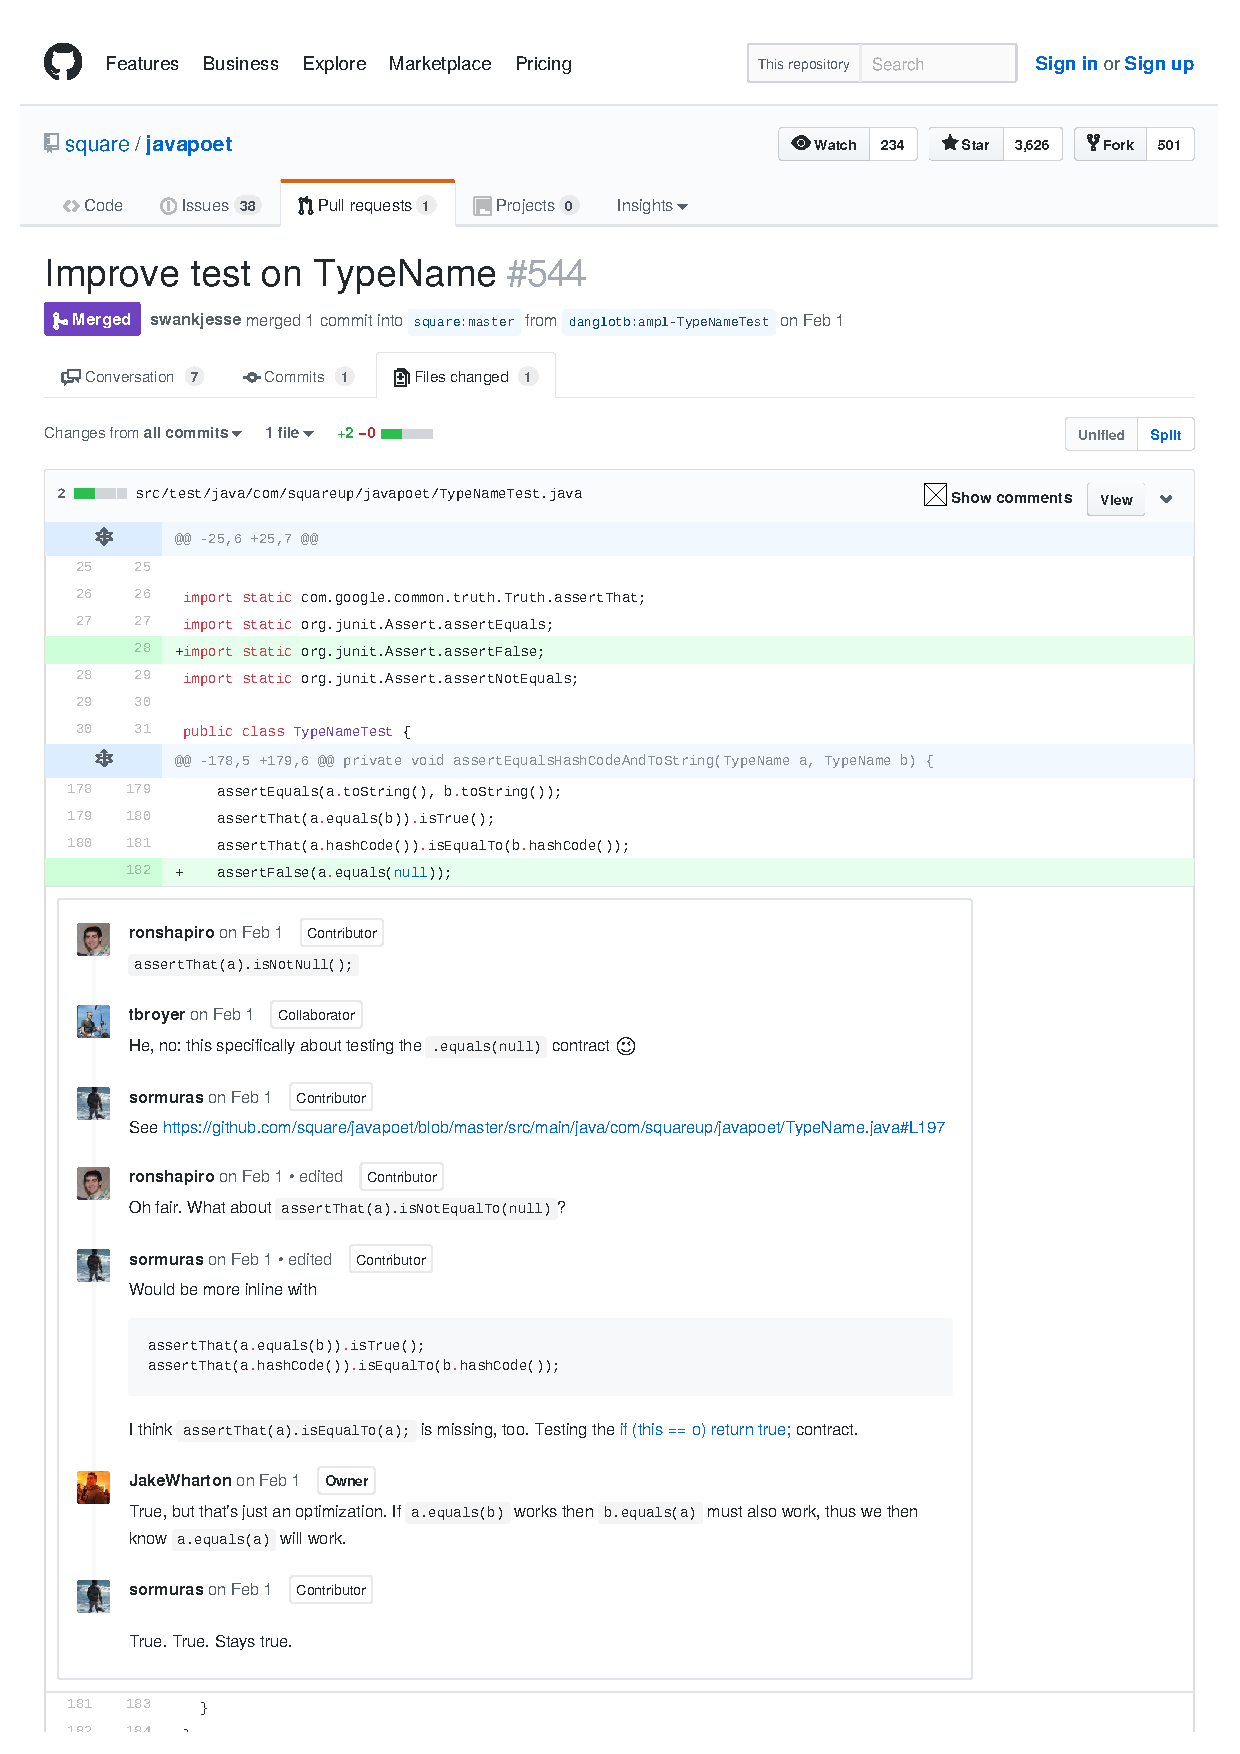
\includegraphics[width=0.98\textwidth, trim=2cm 14.4cm 10.06cm 14.0cm, clip]{javapoet.pdf}}
\end{figure}
The title of the pull resuest is: ``\emph{Improve test on TypeName}'' with the following short text: ``\emph{Hello, I open this pull request to specify the line 197 in the equals() method of com.squareup.javapoet.TypeName. if (o == null) return false;}''
This test improvement synthesized by \dspot has been merged by of the lead developer of javapoet one hour after its proposal.


% -----------------------------------------------------------------------------
% MYBATIS
% -----------------------------------------------------------------------------
\subsubsection{mybatis-3}

% mybatis-3 used: shouldGetAndSetNestedProperty_cf114673
%\todo{MyBatis is a object relational mapper framework (aka ORM). The original test suite kills 75.3\% --- 14821 over 19685 of the mutant generated by \pitest. DATASET}

In project mybatis-3, \dspot has been applied to amplify a test for \texttt{MetaClass}. 
\dspot synthesizes a single assertion that kills 8 more mutants.
All new mutants killed are located between lines 174 and 179, \ie the \texttt{then} branch of an \texttt{if-statement} in method \texttt{buildProperty(String property, StringBuilder sb)} of \texttt{MetaClass}.
This method builds a String that represents the  property given as input. 
The \texttt{then} branch is responsible to build  the String in case the \texttt{property} has a child, \eg the input is ``richType.richProperty''. 
This behavior is not specified at all in the original test class.

I have proposed to the developers the following pull request entitled ``\emph{Improve test on MetaClass}'' with the following short text: ``\emph{Hello, I open this pull request to specify the lines 174-179 in the buildProperty(String, StringBuilder) method of MetaClass.}'' \footnote{\url{https://github.com/mybatis/mybatis-3/pull/912/files}}:
\begin{figure}[H]
	\centering\fbox{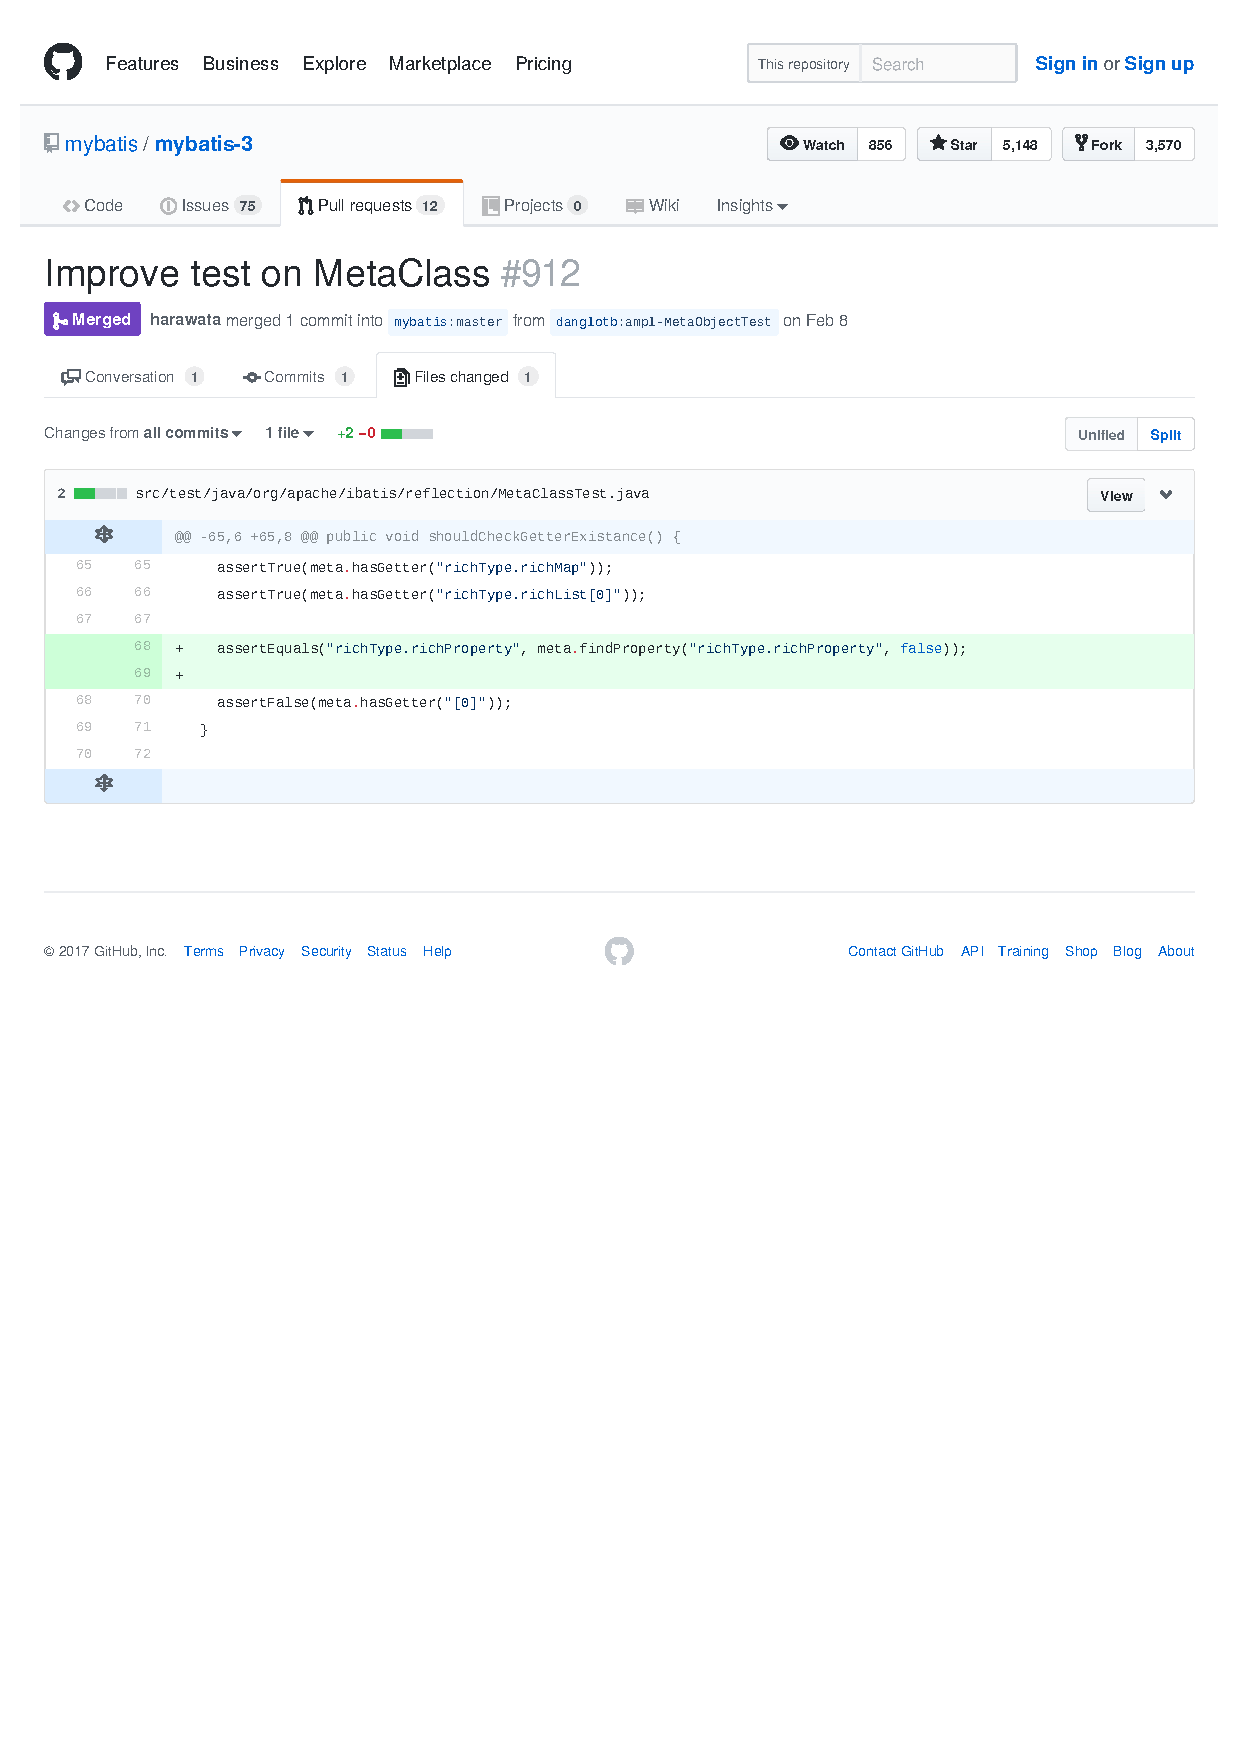
\includegraphics[width=0.98\textwidth, trim=2cm 17.5cm 4.5cm 10.5cm, clip]{mybatis.pdf}}
\end{figure}

The developer accepted the test improvement and merged the pull request the same day without a single objection. 


% -----------------------------------------------------------------------------
% TRACCAR
% -----------------------------------------------------------------------------
\subsubsection{traccar}
% top killer : testDecode_cf39

\dspot has been applied to amplify \texttt{ObdDecoderTest}. 
It identifies a single assertion that kills 14 more mutants.
All newly killed mutants are located between lines 60 to 80, \ie in the method \texttt{decodesCodes()} of \texttt{ObdDecoder}, which is responsible to decode a \texttt{String}. 
In this case, the pull request consists of a new test method because the new assertions do not fit with the intent of existing tests. 
This new test method is proposed into \texttt{ObdDecoderTest}, which is the class under amplification. 
The PR was entitled ``\emph{Improve test cases on ObdDecoder}'' with the following description: ``\emph{Hello, I open this pull request to specify the method decodeCodes of the ObdDecoder}''. \footnote{\url{https://github.com/tananaev/traccar/pull/2897}}
\begin{figure}[H]
	\centering\fbox{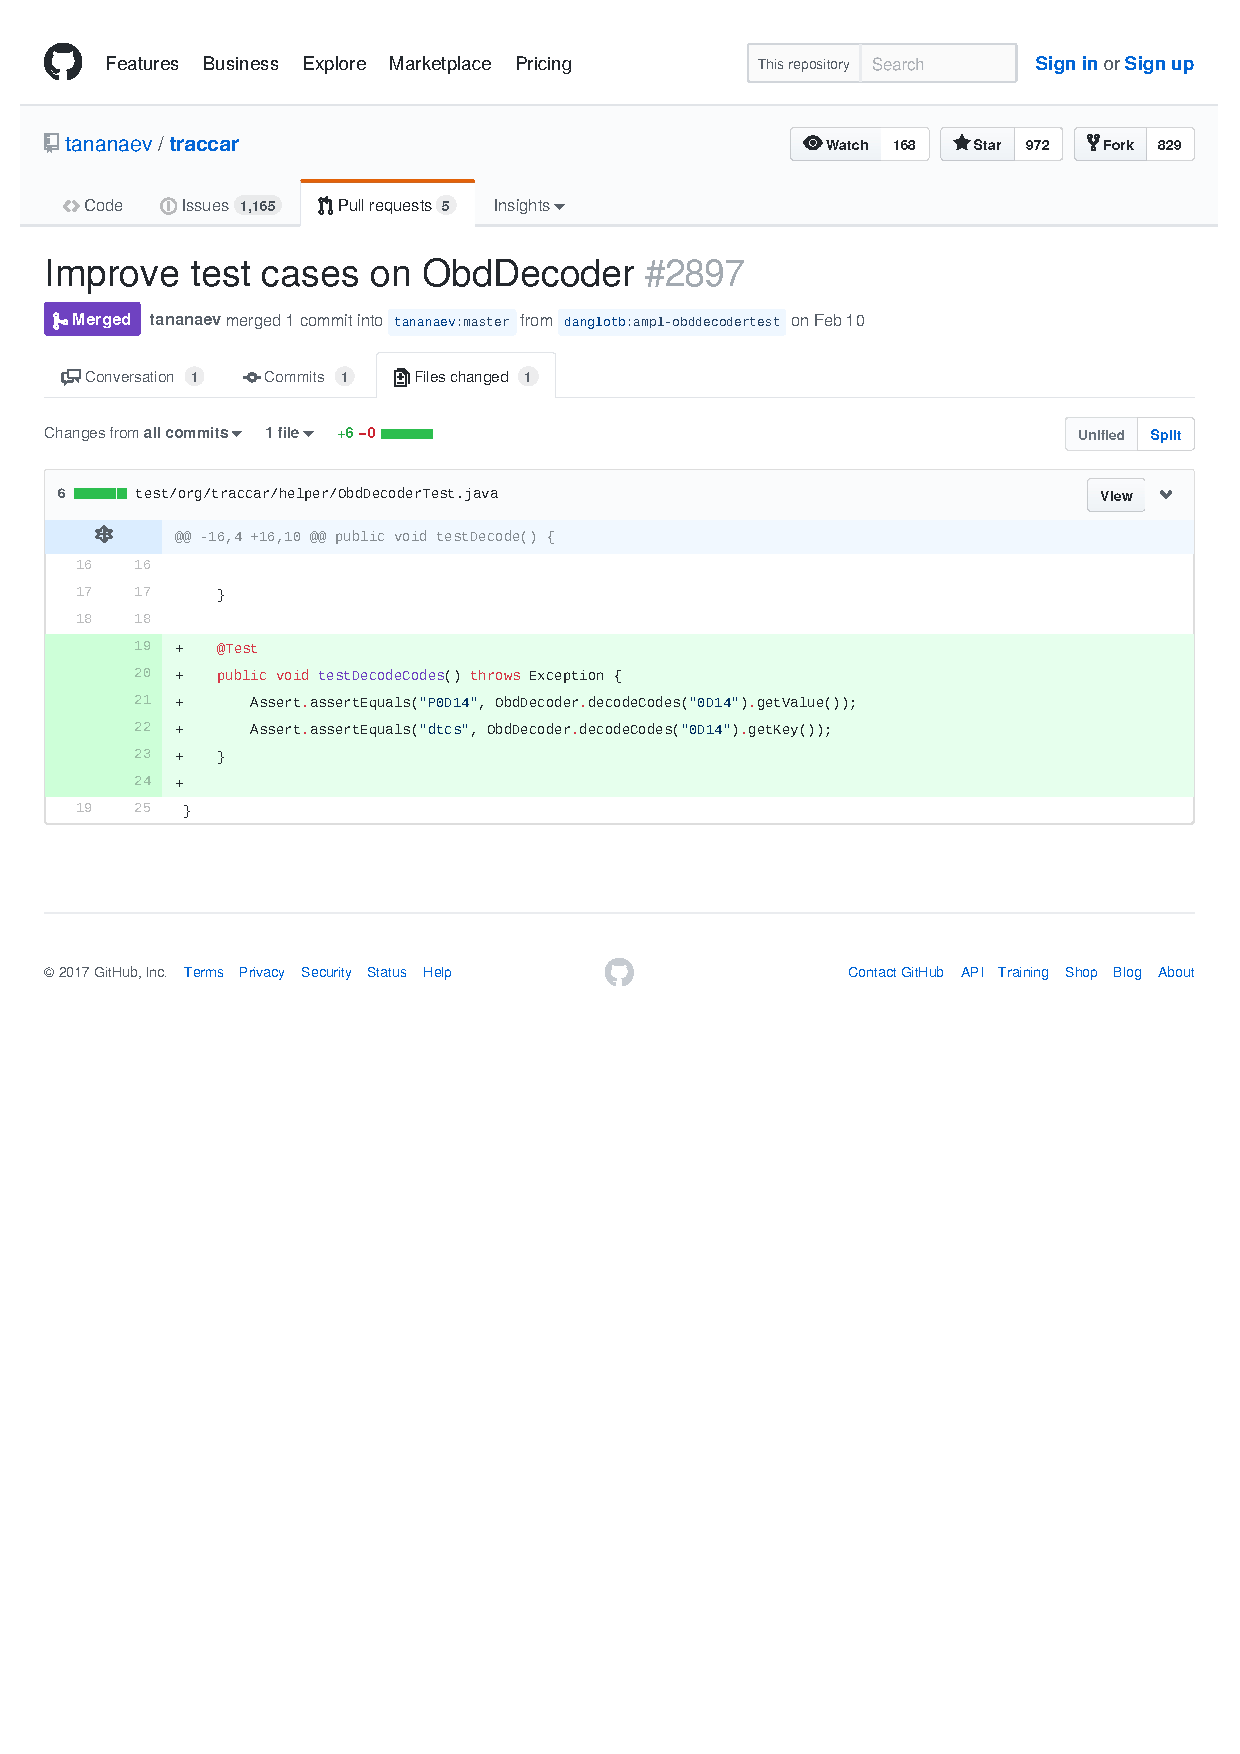
\includegraphics[width=0.98\textwidth, trim=2cm 15.57cm 6.35cm 9.88cm, clip]{traccar.pdf}}
\end{figure}

The developer of traccar thanked us for the proposed changes and merged it the same day.


% -----------------------------------------------------------------------------
% STREAM LIB
% -----------------------------------------------------------------------------
\subsubsection{stream-lib}

%testHash64ByteArrayOverload_cf92

% https://github.com/addthis/stream-lib/pull/128/files

\dspot has been applied to amplify \texttt{TestMurmurHash}. 
It identifies a new test input that kills 15 more mutants.
All newly killed mutants are located in method \texttt{hash64()} of \texttt{MurmurHash} from lines 158 to 216.
 This method computes a hash for a given array of byte. 
 The PR was entitled ``\emph{Test: Specify hash64}'' with the following description: ``\emph{The proposed change specifies what the good hash code must be. With the current test, any change in "hash" would still make the test pass, incl. the changes that would result in an inefficient hash.}''. \footnote{\url{https://github.com/addthis/stream-lib/pull/127/files}}:
\begin{figure}[H]
	\centering\fbox{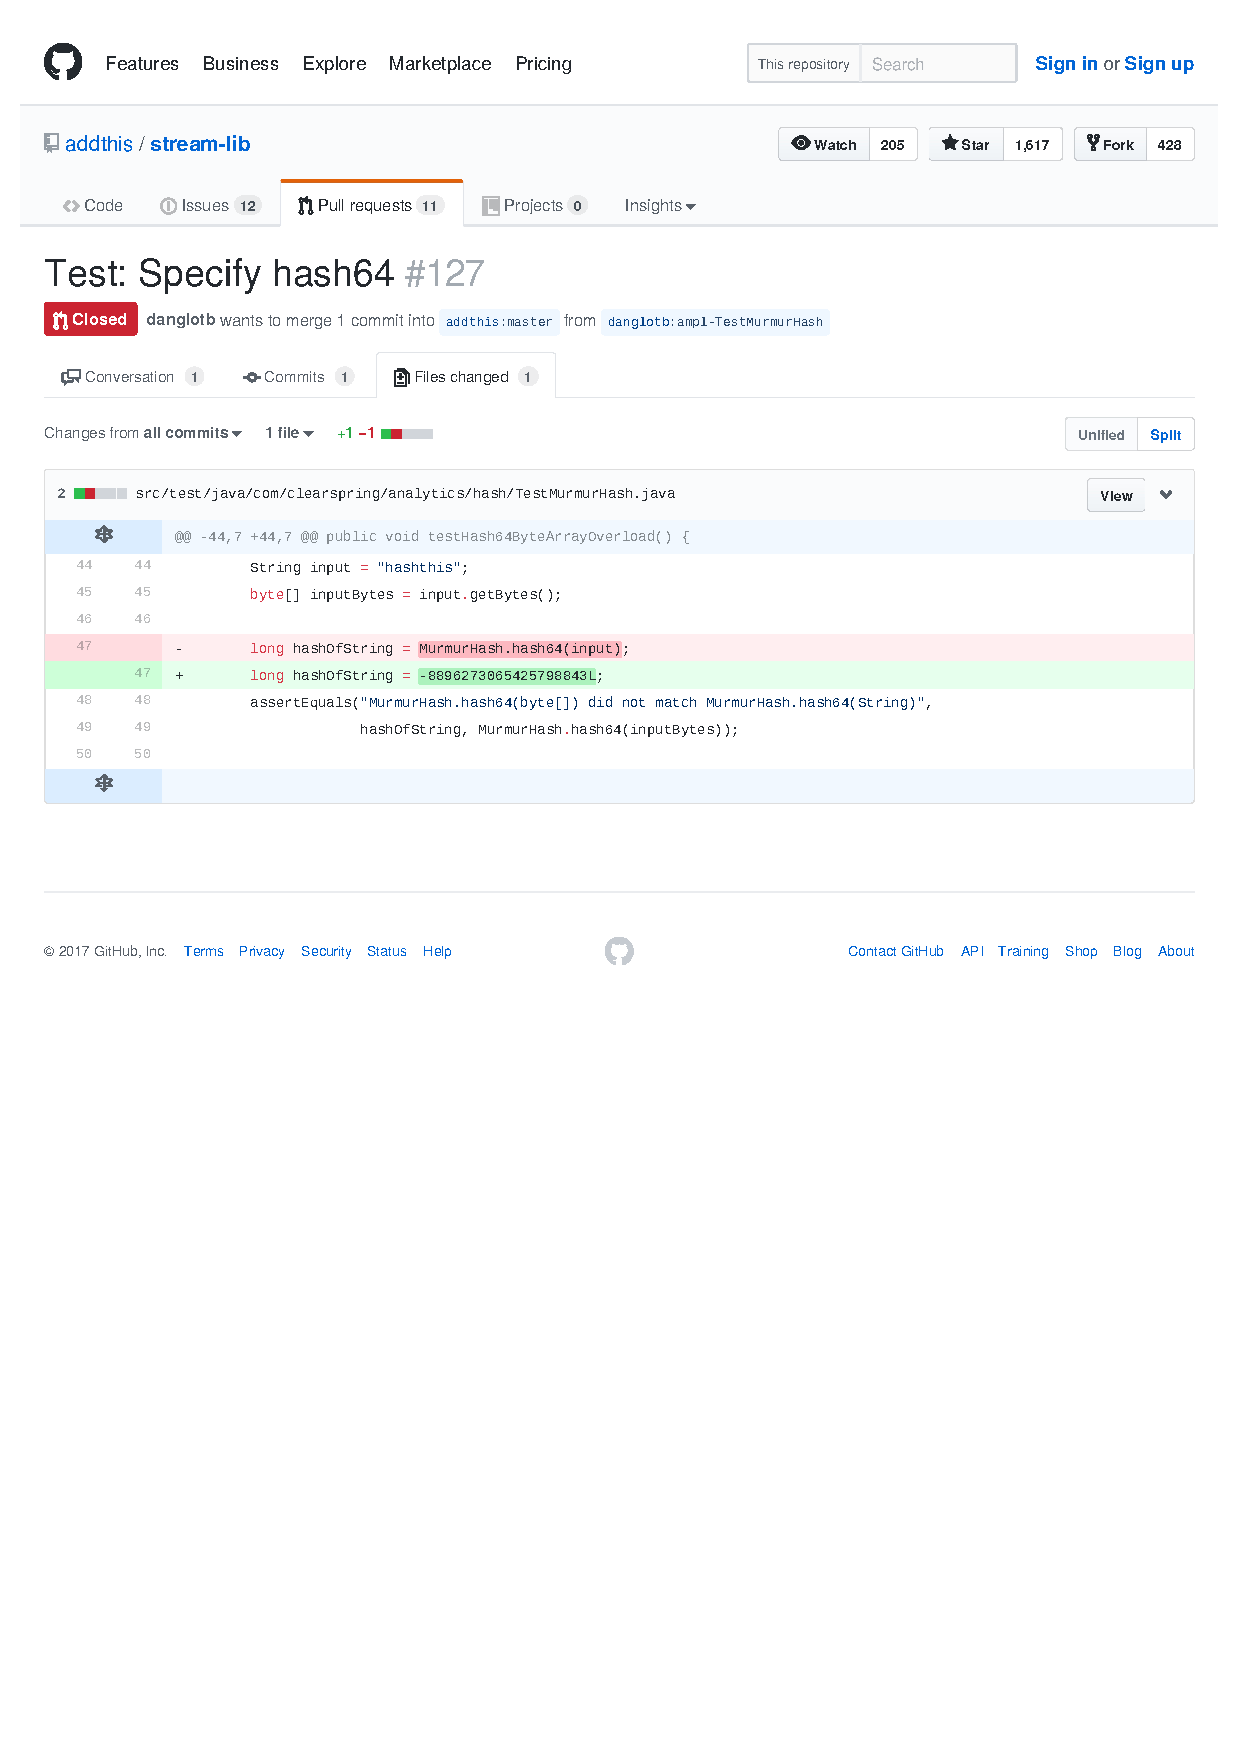
\includegraphics[width=0.98\textwidth, trim=2cm 17.07cm 4.90cm 10.59cm, clip]{stream-lib0.pdf}}
\end{figure}

Two days later, one developer mentioned the fact that the test is verifying the overload of the method and is not specifying the method hash itself. 
He closed the PR because it was not relevant to put changes there. 
He suggested to open an new pull request with a new test method instead of changing the existing test method. 
I proposed, 6 days later, a second pull request entitled ``\emph{add test for hash() and hash64() against hard coded values}'' with no description, since we estimated that the developer was aware of our intention.\footnote{\url{https://github.com/addthis/stream-lib/pull/128/files}}:
\begin{figure}[H]
	\centering\fbox{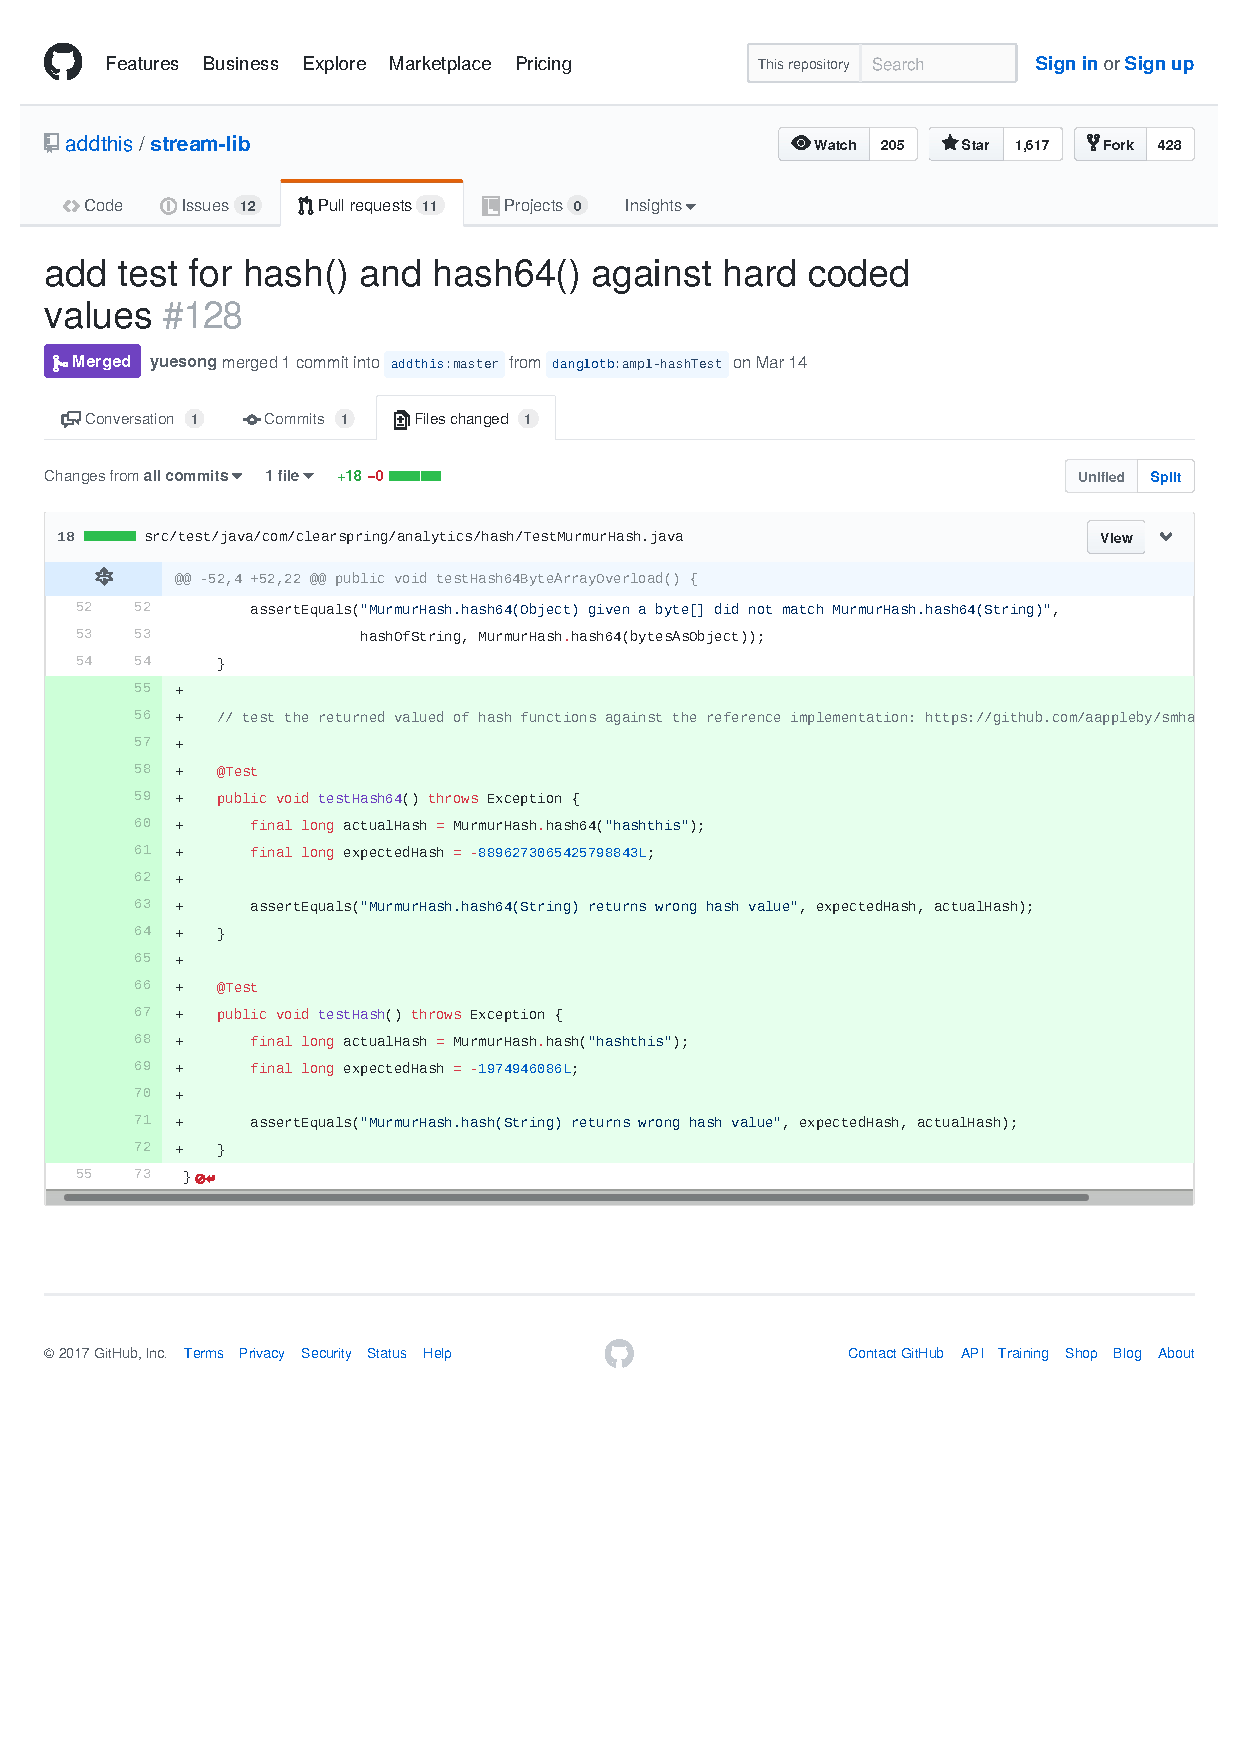
\includegraphics[width=0.98\textwidth, trim=2cm 9.55cm 3.35cm 11.02cm, clip]{stream-lib.pdf}}
\end{figure}

The pull request has been merged by the same developer 20 days later.


% -----------------------------------------------------------------------------
% MUSTACHE.JAVA
% -----------------------------------------------------------------------------
\subsubsection{mustache.java}

%testAbstractClass_add3_literalMutation38_literalMutation326_failAssert19

\dspot has been applied to amplify \texttt{AbstractClassTest}. 
It identifies a try/catch/fail block that kills 2 more mutants.
This is an interesting new case, compared to the ones previously discussed, because it is about the specification of exceptions, \ie of behavior under erroneous inputs.
All newly killed mutants are located in method \texttt{compile()} on line 194.
 The test specifies that if a variable is improperly closed, the program must throw a \texttt{MustacheException}. 
 In the Mustache template language, an improperly closed variable occurs when an opening brace ``$\{$'' does not have its matching closing brace such as in the input of the proposed changes. 
 We propose the pull request to the developers, entitled ``\emph{Add Test: improperly closed variable}'' with the following description: ``\emph{Hello, I proposed this change to improve the test on MustacheParser. When a variable is improperly closed, a MustacheException is thrown.}''.\footnote{\url{https://github.com/spullara/mustache.java/pull/186/files}}
\begin{figure}[H]
	\centering\fbox{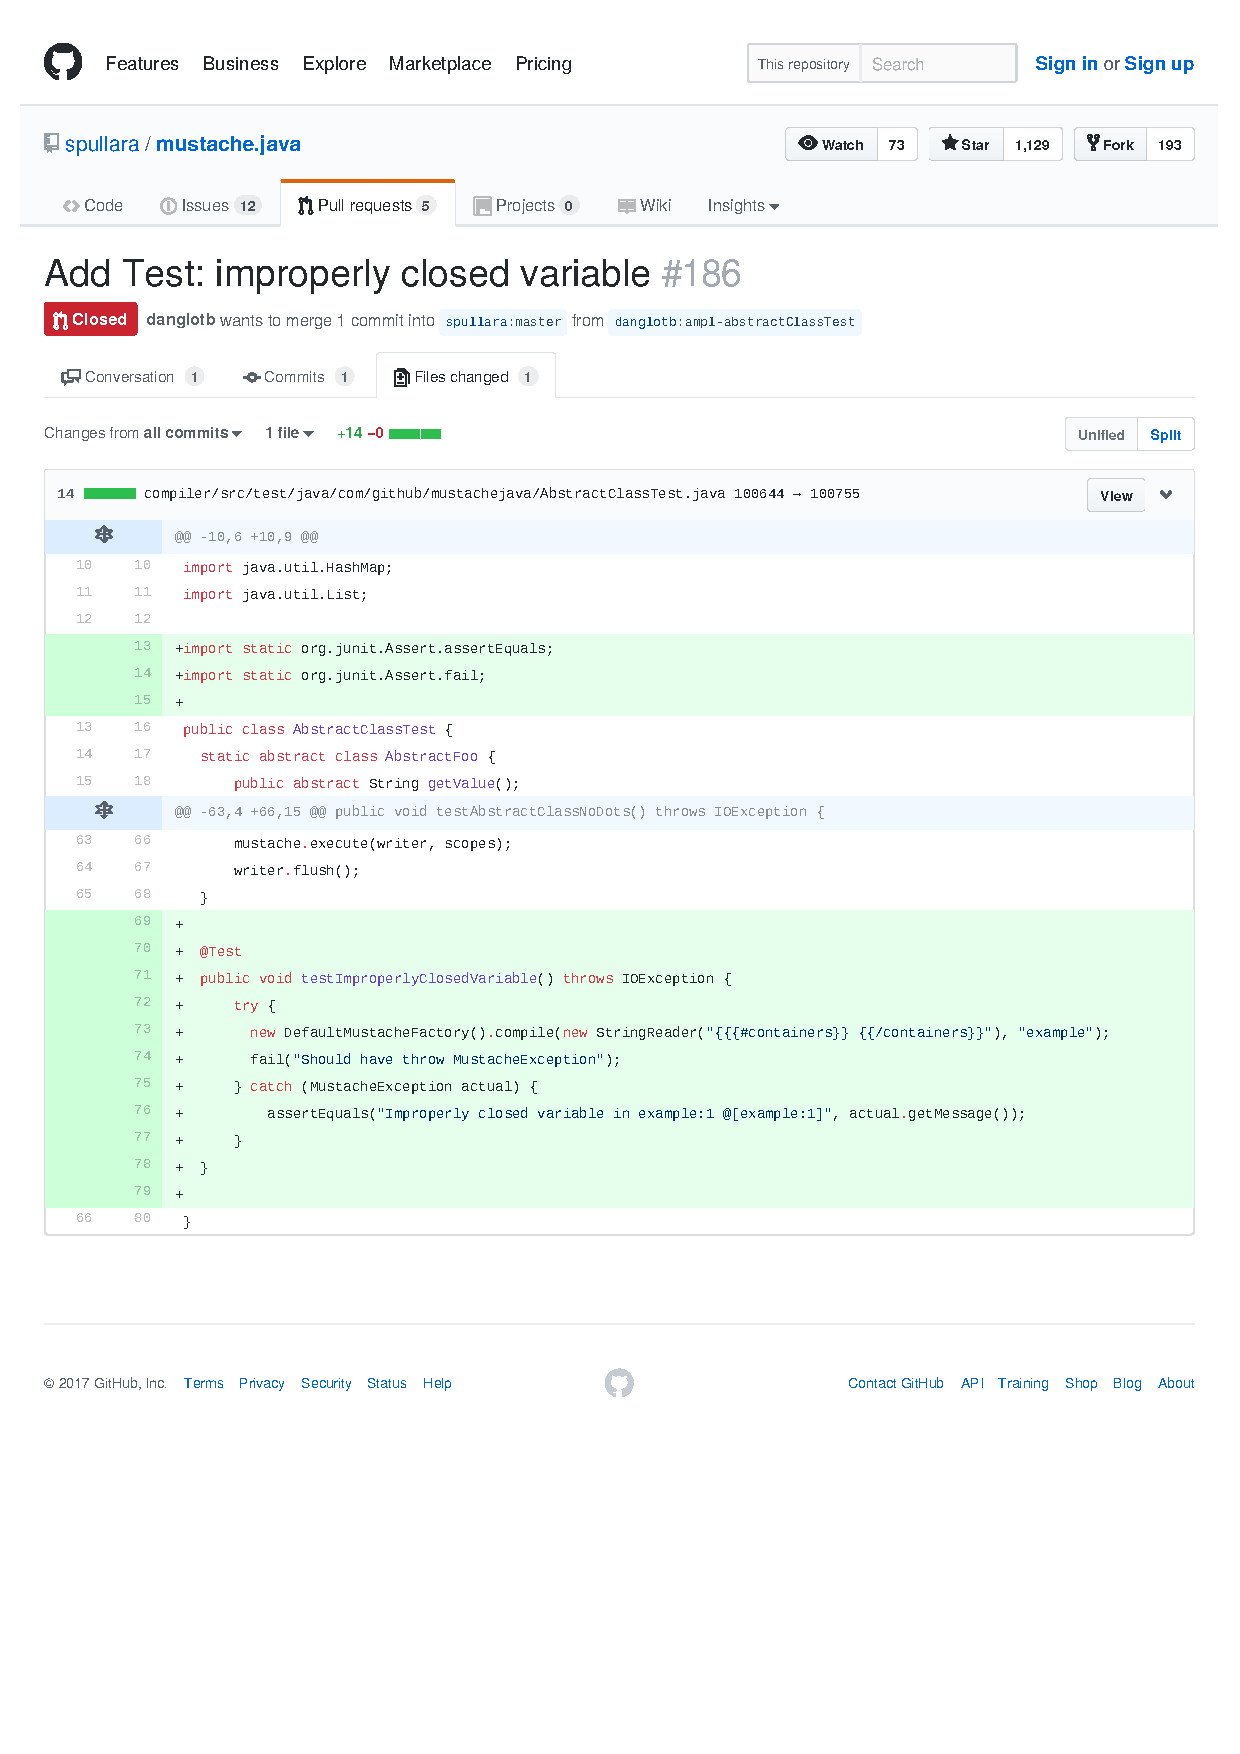
\includegraphics[width=0.98\textwidth, trim=2cm 8.86cm 2.03cm 14.96cm, clip]{mustache-java.pdf}}
\end{figure}

12 days later, a developer accepted the change, but noted that the test should be in another class.
 He closed the pull request and added the changes himself into the desired class.\footnote{the diff is same:\url{https://github.com/spullara/mustache.java/commit/9efa19d595f893527ff218683e70db2ae4d8fb2d}}. 

% -----------------------------------------------------------------------------
% TWILIO-JAVA
% -----------------------------------------------------------------------------
\subsubsection{twilio-java}

\dspot has been applied to amplify \texttt{RequestTest}. 
It identifies two new assertions that kill 4 more mutants. 
All mutants were created between lines 260 and 265 in the method \texttt{equals()} of \texttt{Request}. 
The change specifies that an object \texttt{Request} is not equal to null nor an object of different type, \ie \texttt{Object} here. 
The pull request was entitled ``\emph{add test equals() on request}'', accompanied with the short description ``\emph{Hi, I propose this change to specify the equals() method of com.twilio.http.Request, against object and null value}'' \footnote{\url{https://github.com/twilio/twilio-java/pull/334/files}}:
\begin{figure}[H]
	\centering\fbox{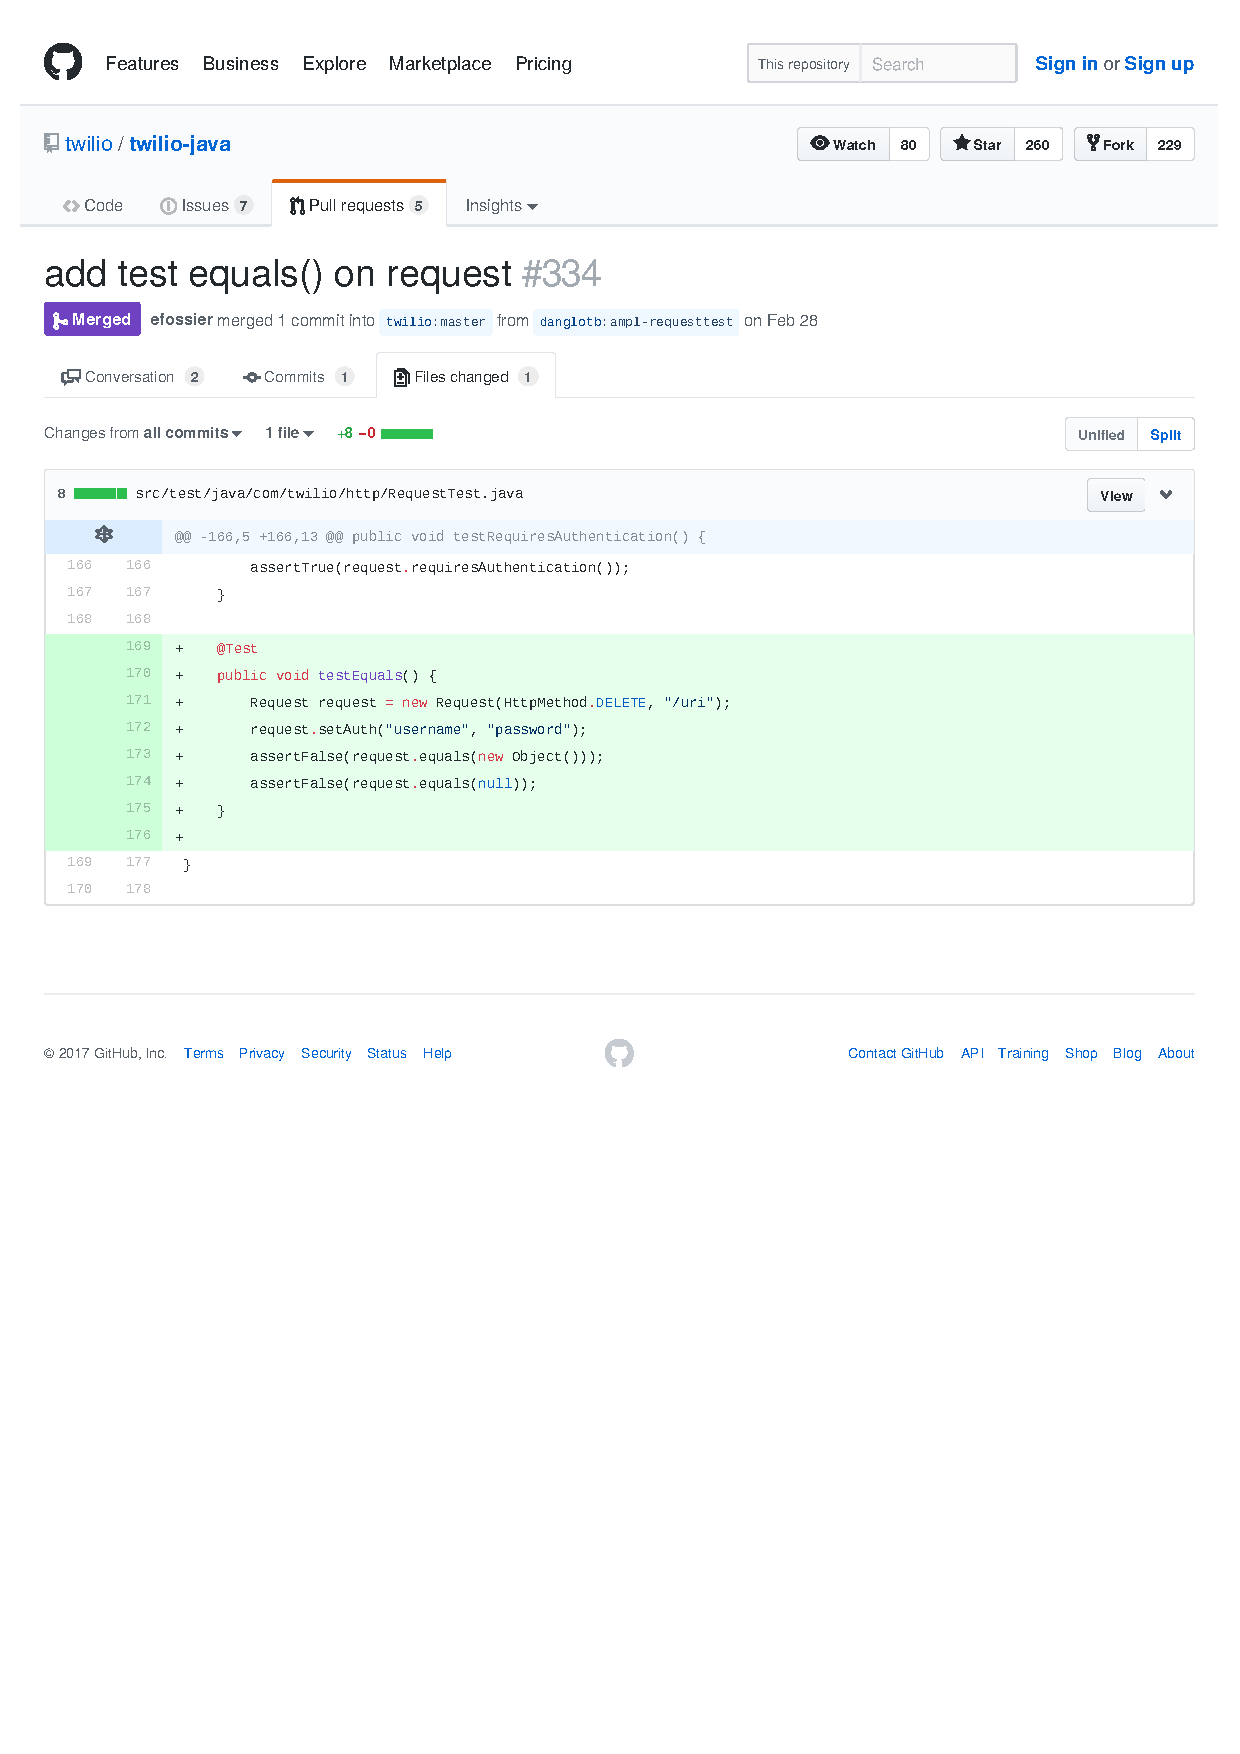
\includegraphics[width=0.98\textwidth, trim=2cm 14.83cm 8.11cm 10.11cm, clip]{twilio-java.pdf}}
\end{figure}

A developer merged the change 4 days later.

% 
% 25 minutes
% testGetUsername_cf47548_cf49619_cf53871
% best fitness, all mutant are killed in equals pr easy to build
% adding assertion manually against null, for having a complete test case.

% ExcludedClasses = com.twilio.http.NetworkHttpClientTest

% -----------------------------------------------------------------------------
% JSOUP
% -----------------------------------------------------------------------------
\subsubsection{jsoup}

\dspot has been applied to amplify \texttt{AttributeTest}. 
It identifies one assertion that kills 13 more mutants.
 All mutants are in the method \texttt{hashcode} of Attribute. 
 The pull request was entitled ``\emph{add test case for hashcode in attribute}'' with the following short description ``\emph{Hello, I propose this change to specify the hashCode of the object org.jsoup.nodes.Attribute.}''\footnote{\url{https://github.com/jhy/jsoup/pull/840}}:
\begin{figure}[H]
	\centering\fbox{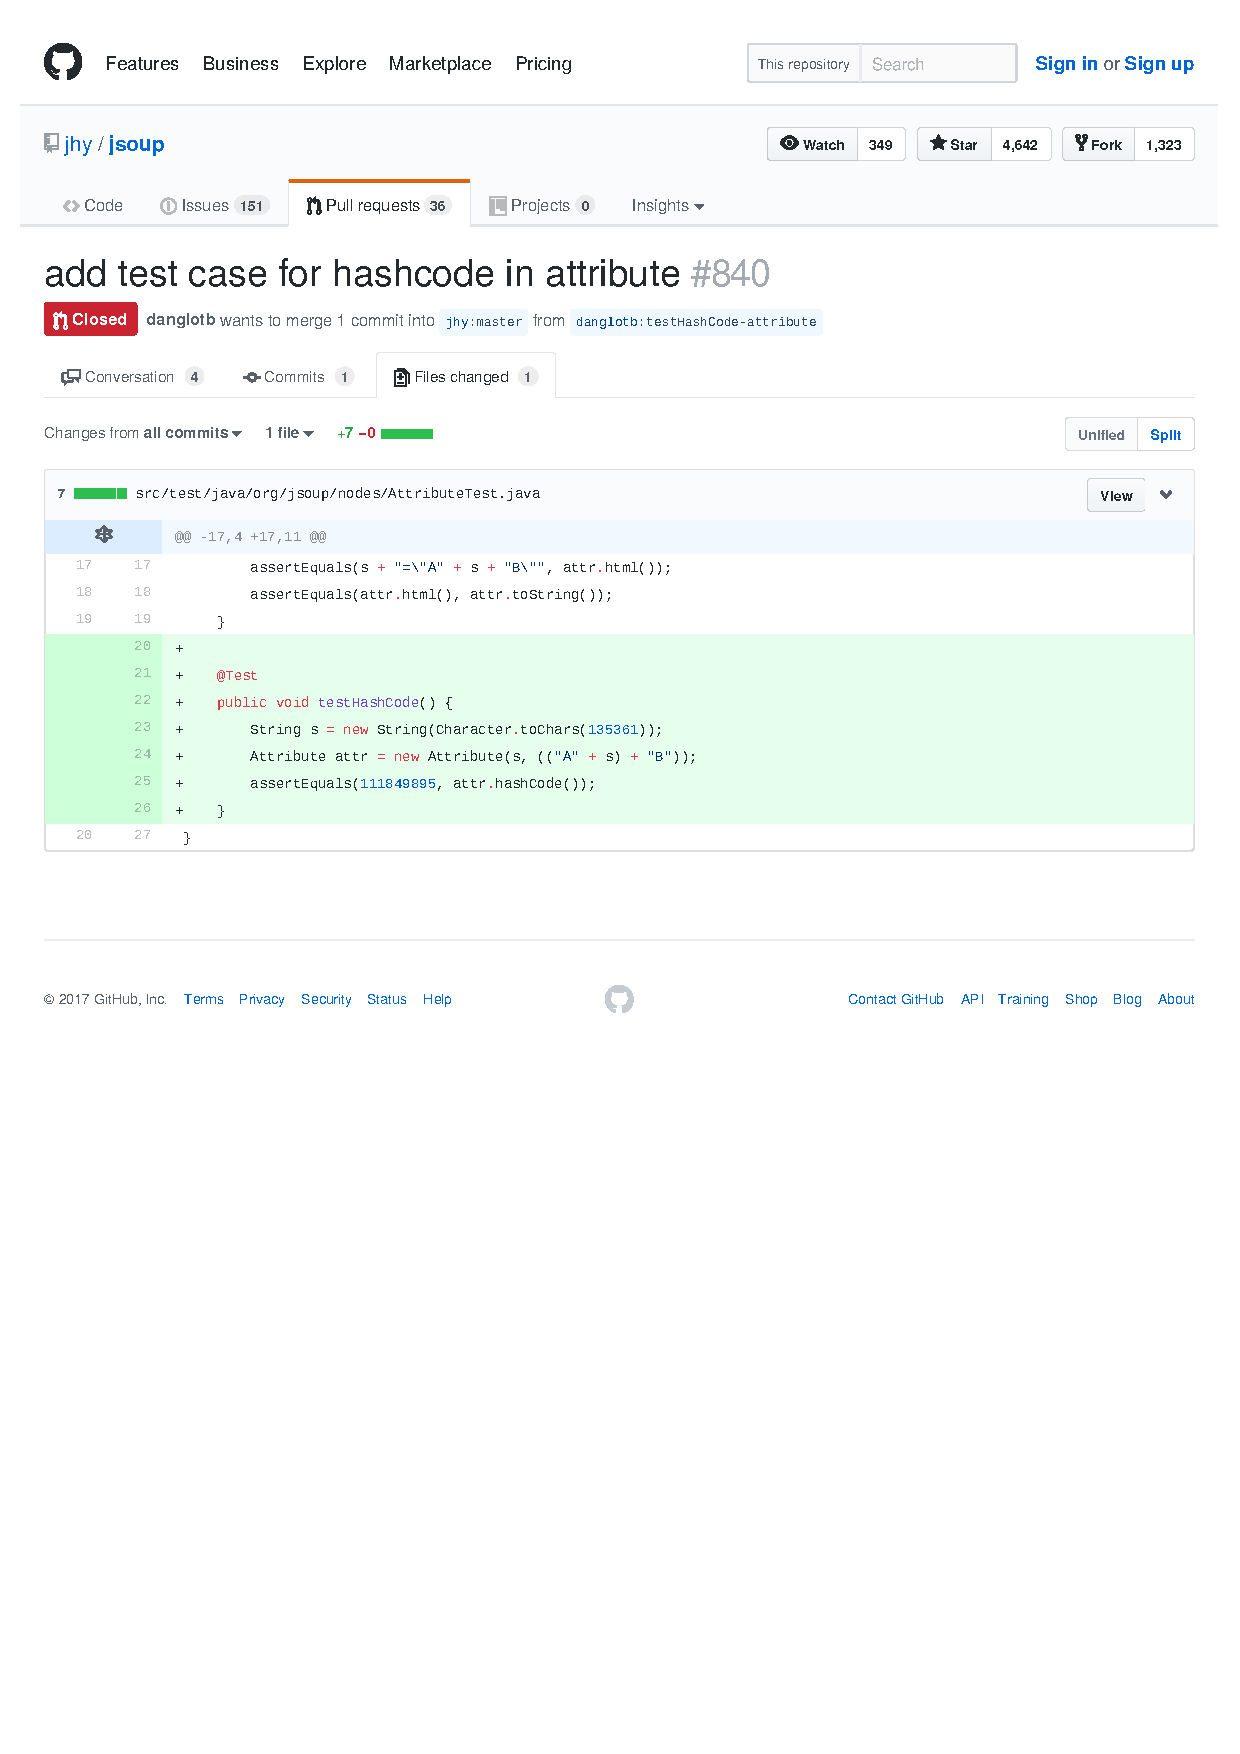
\includegraphics[width=0.98\textwidth, trim=2cm 15.5cm 9cm 10.4cm, clip]{jsoup.pdf}}
\end{figure}

One developer highlighted the point that the \texttt{hashCode} method is an implementation detail, and it is not a relevant element of the API. 
Consequently, he did not accept our test improvement.

At this point, I have made two pull requests targeting \texttt{hashCode} methods. 
One accepted and one rejected. 
\texttt{hashCode} methods could require a different testing approach to validate the number of potential collisions in a collection of objects rather than checking or comparing the values of a few objects created for one explicit test case. The different responses we obtained reflect the fact that developer teams and policies ultimately decide how to test the hash code protocol and the outcome could be different from different projects.

%\TODO{I don't know if i disagree with this developer now, because the contract should be tested not the values.}
%We disagree with this developer, and think that \texttt{hashCode} methods are worth a test case, because the contracts of \texttt{hashCode} methods are essential for many high-level usages such as collection usages. However, we would agree that such generic test cases may be generated by a dedicated testing framework.


% -----------------------------------------------------------------------------
% PROTOSTUFF
% -----------------------------------------------------------------------------
\subsubsection{protostuff}

\dspot has been applied to amplify \texttt{TailDelimiterTest}. 
It identifies a single assertion that kills 3 more mutants.
All new mutants killed are in the method \texttt{writeTo} of \texttt{ProtostuffIOUtil} on lines 285 and 286, which is responsible to write a buffer into a given scheme. 
I proposed a pull request entitled ``\emph{assert the returned value of writeList}'', with the following short description ``\emph{Hi, I propose the following changes to specify the line 285-286 of io.protostuff.ProtostuffIOUtil.}''\footnote{\url{https://github.com/protostuff/protostuff/pull/212/files}}, shown earlier in \autoref{fig:diff-protostuff}

\begin{figure}[H]
	\centering\fbox{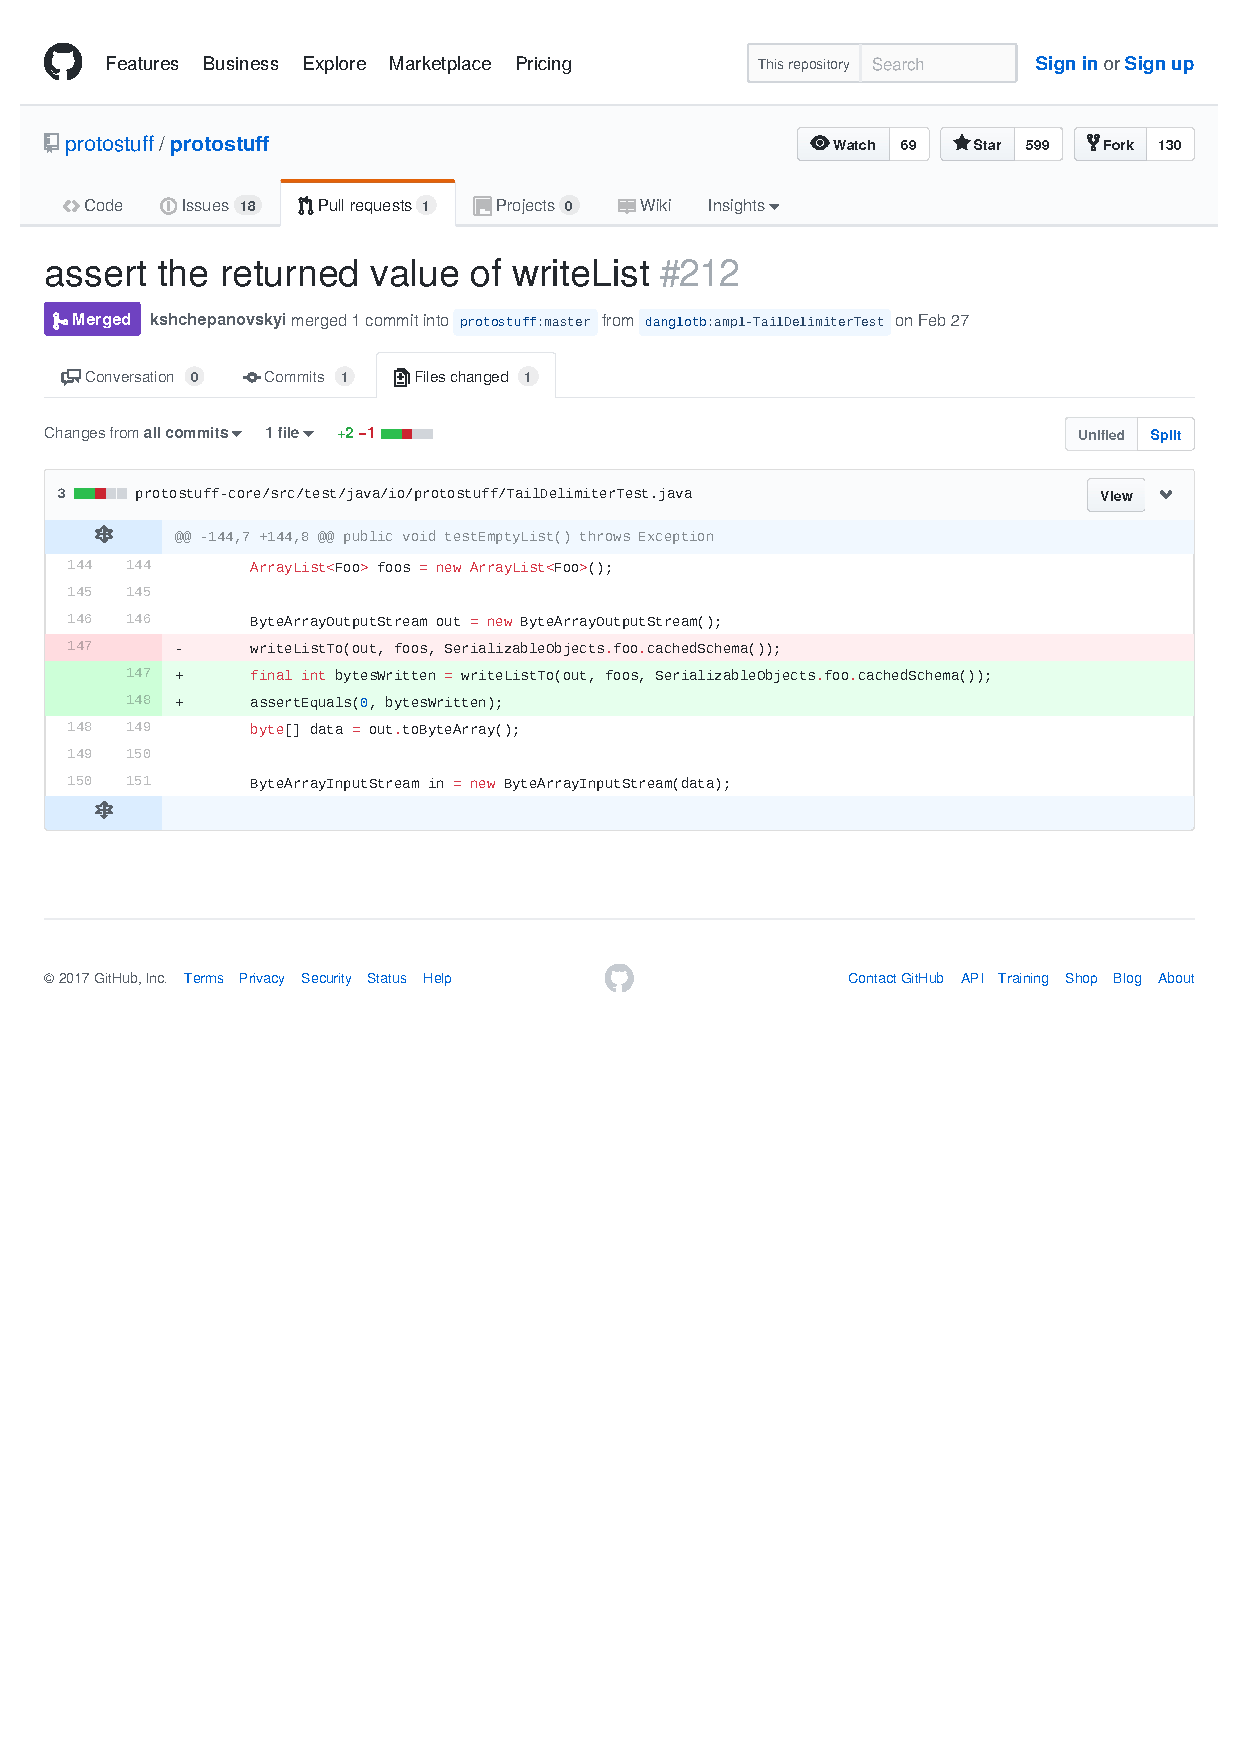
\includegraphics[width=0.98\textwidth, trim=2cm 16.3cm 4cm 10.4cm, clip]{protostuff.pdf}}
\end{figure}

A developer accepted the proposed changes the same day.

%testEmptyList_add5651

% -----------------------------------------------------------------------------
% LOGBACK
% -----------------------------------------------------------------------------
\subsubsection{logback}

\dspot has been applied to amplify \texttt{FileNamePattern}. 
It identifies a single assertion that kills 5 more mutant. 
Newly killed mutants were located at lines 94, 96 and 97 of the \texttt{equals} method of the \texttt{FileNamePattern} class. 
The proposed pull request was entitle ``\emph{test: add test on equals of FileNamePattern against null value}'' with the following short description: ``\emph{Hello, I propose this change to specify the equals() method ofFileNamePattern against null value}''.\footnote{\url{https://github.com/qos-ch/logback/pull/365/files}}:

\begin{figure}[H]
	\centering\fbox{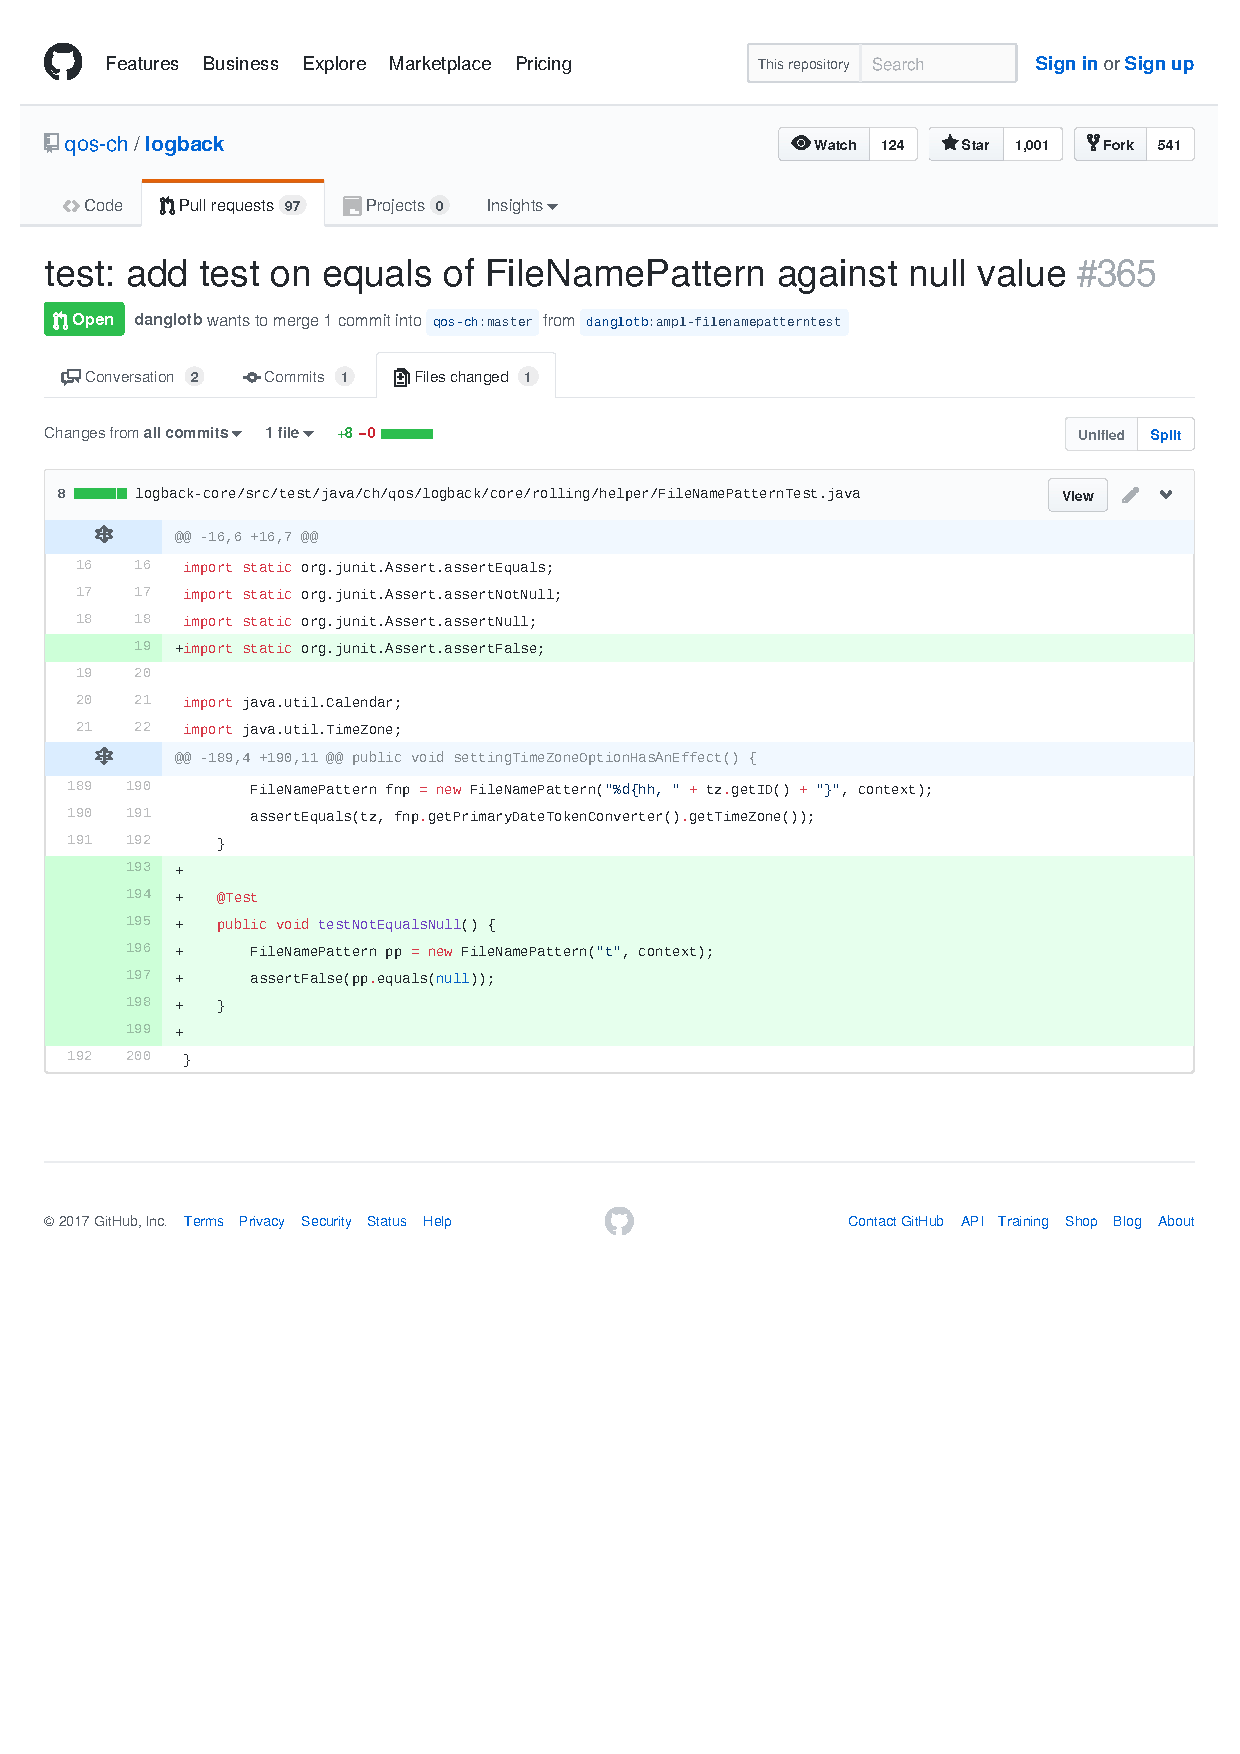
\includegraphics[width=0.98\textwidth, trim=2cm 11.66cm 8.69cm 14.20cm, clip]{logback.pdf}}
\end{figure}

Even if the test asserts the contract that the \texttt{FileNamePattern} is not equals to null, and kills 5 more mutants, the lead developer does not get the point to test this behavior. 
The pull request has not been accepted.

%testSmoke_cf69003

% -----------------------------------------------------------------------------
% RETROFIT
% -----------------------------------------------------------------------------
\subsubsection{retrofit}

I did not manage to create a pull request based on the amplification of the test suite of retrofit. 
According to the result, the newly killed mutants are spread over all the code, and thus the amplified methods did not identify a missing contract specification. 
This could be explained by two facts: 
1) the original test suite of retrofit is strong: there is no test class with low \ms and a lot of them are very high \ms, \ie 90\% and more;
2) the original test suite of retrofit uses complex test mechanism such as mock and fluent assertions of the form the \texttt{assertThat().isSomething()}. 
For the former point, it means that \dspot has been able to improve, even a bit, the \ms of a very strong test suite, but not in targeted way that makes sense in a pull request.
For the latter point, this puts in evidence the technical challenge of amplifying fluent assertions and mocking mechanisms.

~\\

%% new section for rev2.13
\subsubsection{Contributions of \Aampl and \Iampl to the Pull-requests}

\begin{table}[]
	\caption{Contributions of \Aampl and \Iampl on the amplified test method used to create a pull request.}
	\label{tab:contrib-a-i-ampl}
	\centering\begin{tabular}{lcc}
		\hline
		Project & \#\Aampl &  \#\Iampl \\
		\hline
		javapoet & 2 & 2 \\
		mybatis-3 & 3 & 3 \\
		traccar & 10 & 7 \\
		stream-lib & 2 & 2 \\
		mustache & 4 & 3 \\
		twilio & 3 & 4 \\
		jsoup & 34 & 0 \\
		protostuff & 1 & 1 \\
		logback & 2 & 2 \\
		\hline
	\end{tabular}
\end{table}

In \autoref{tab:contrib-a-i-ampl}, I summarize the contribution of \Aampl and \Iampl, where a contribution means an source code modification added during the main amplification loop. 
In 8 cases over the 9 pull-requests, both \Aampl and \Iampl were necessary. 
Only the pull request on jsoup was found using only \Aampl. 
This means that for all the other pull-requests, the new inputs were required to be able: 
1) to kill new mutants and 
2) to obtain amplified test methods that have values for the developers.

Note that this does not contradict with the fact that the pull-requests are one-liners.
Most one-liner pull-requests contain both a new assertion and a new input. Consider the following Javapoet's one liner \texttt{assertFalse(x.equals(null))} (javapoet). 
In this example, although there is a single line starting with ``assert'', there is indeed a new input, the value ``null''.

~\\
~\\
\begin{mdframed}
	\textit{\rqpullrequest: Would developers be ready to permanently accept improved test cases into the test repository?}\\
	Answer: 19 test improvements have been proposed to developers of notable open-source projects. 
	13/19 have been considered valuable and have been merged into the main test suite. 
	The developers' feedback has confirmed the relevance, and also the challenges of automated test improvement.
\end{mdframed}

In the area of automatic test improvement, this experiment is the first to put real developers in the loop, by asking them about the quality of automatically improved test cases.
To the best of my knowledge, this is the first public report of automatically improved tests accepted by unbiased developers and merged in the master branch of open-source repositories.

\begin{table}
	\caption{The effectiveness of test amplification with \dspot on 40 test classes: 24 well-tested (upper part) and 16 average-tested (lower part) real test classes from notable open-source Java projects.}
	%A star after a test name means that the test is considered as subject for the relevance study of \rqpullrequest.}
	\label{tab:overall-results}
	\def\arraystretch{0.55}%  1 is the default, change whatever you need
	\setlength\tabcolsep{0.45pt} % default value: 6pt
	\small
	\begin{tabular}{|llrrrr|rrrr|rrr|r|}
		\rotverticalinv{ID}&
		\rotverticalinv{Class}&
		\rotverticalinv{\# Orig. test methods}&
		\rotverticalinv{Mutation Score}&
		\rotverticalinv{\# New test methods}&
		\rotverticalinv{\begin{tabular}{l}
				Candidates \\ for pull request
		\end{tabular}}&
		\rotverticalinv{\# Killed mutants orig.}&
		\rotverticalinv{\# Killed mutants ampl.}&
		\rotverticalinv{Increase killed}&
		&%arrow for killed
		\setlength{\tabcolsep}{0cm} 
		\rotverticalinv{\begin{tabular}{l}
				\# Killed mutants only\\ A-ampl
		\end{tabular}}&
		\setlength{\tabcolsep}{0cm} 
		\rotverticalinv{\begin{tabular}{l}
				Increase killed only\\ A-ampl
		\end{tabular}}&
		&%arrow for killed
		\rotverticalinv{Time (minutes)}\\
		\hline\\
		&\multicolumn{3}{l}{High \ms}\\
		\hline\\
		1&\scriptsize{TypeNameTest}&12&50\%&19&8&599&715&19\%&{\color{ForestGreen}$\nearrow$}&599&0.0\%&$\rightarrow$&11.11 \\
		\rowcolor[HTML]{EFEFEF}
		2&\scriptsize{NameAllocatorTest}&11&87\%&0&0&79&79&0.0\%&$\rightarrow$&79&0.0\%&$\rightarrow$&4.76 \\
		3&\scriptsize{MetaClassTest}&7&58\%&108&10&455&534&17\%&{\color{ForestGreen}$\nearrow$}&455&0.0\%&$\rightarrow$&235.71 \\
		\rowcolor[HTML]{EFEFEF}
		4&\scriptsize{ParameterExpressionTest}&14&91\%&2&2&162&164&1\%&{\color{ForestGreen}$\nearrow$}&162&0.0\%&$\rightarrow$&25.93 \\
		5&\scriptsize{ObdDecoderTest}&1&80\%&9&2&51&54&5\%&{\color{ForestGreen}$\nearrow$}&51&0.0\%&$\rightarrow$&2.20 \\
		\rowcolor[HTML]{EFEFEF}
		6&\scriptsize{MiscFormatterTest}&1&72\%&5&5&42&47&11\%&{\color{ForestGreen}$\nearrow$}&42&0.0\%&$\rightarrow$&1.21 \\
		7&\scriptsize{TestLookup3Hash}&2&95\%&0&0&464&464&0.0\%&$\rightarrow$&464&0.0\%&$\rightarrow$&6.76 \\
		\rowcolor[HTML]{EFEFEF}
		8&\scriptsize{TestDoublyLinkedList}&7&92\%&1&1&104&105&0.97\%&{\color{ForestGreen}$\nearrow$}&104&0.0\%&$\rightarrow$&3.03 \\
		9&\scriptsize{ArraysIndexesTest}&1&53\%&15&4&576&647&12\%&{\color{ForestGreen}$\nearrow$}&586&1\%&{\color{ForestGreen}$\nearrow$}&10.58 \\
		\rowcolor[HTML]{EFEFEF}
		10&\scriptsize{ClasspathResolverTest}&10&67\%&0&0&50&50&0.0\%&$\rightarrow$&50&0.0\%&$\rightarrow$&4.18 \\
		11&\scriptsize{RequestTest}&17&81\%&4&3&141&156&10\%&{\color{ForestGreen}$\nearrow$}&141&0.0\%&$\rightarrow$&60.55 \\
		\rowcolor[HTML]{EFEFEF}
		12&\scriptsize{PrefixedCollapsibleMapTest}&4&96\%&0&0&54&54&0.0\%&$\rightarrow$&54&0.0\%&$\rightarrow$&13.28 \\
		13&\scriptsize{TokenQueueTest}&6&69\%&18&6&152&165&8\%&{\color{ForestGreen}$\nearrow$}&152&0.0\%&$\rightarrow$&15.61 \\
		\rowcolor[HTML]{EFEFEF}
		14&\scriptsize{CharacterReaderTest}&19&79\%&71&9&309&336&8\%&{\color{ForestGreen}$\nearrow$}&309&0.0\%&$\rightarrow$&57.06 \\
		15&\scriptsize{TailDelimiterTest}&10&71\%&1&1&381&384&0.79\%&{\color{ForestGreen}$\nearrow$}&381&0.0\%&$\rightarrow$&12.90 \\
		\rowcolor[HTML]{EFEFEF}
		16&\scriptsize{LinkBufferTest}&3&48\%&12&7&66&90&36\%&{\color{ForestGreen}$\nearrow$}&66&0.0\%&$\rightarrow$&3.24 \\
		17&\scriptsize{FileNamePatternTest}&12&58\%&27&9&573&686&19\%&{\color{ForestGreen}$\nearrow$}&573&0.0\%&$\rightarrow$&25.08 \\
		\rowcolor[HTML]{EFEFEF}
		18&\scriptsize{SyslogAppenderBaseTest}&1&95\%&1&1&143&148&3\%&{\color{ForestGreen}$\nearrow$}&143&0.0\%&$\rightarrow$&7.88 \\
		19&\scriptsize{RequestBuilderAndroidTest}&2&99\%&0&0&513&513&0.0\%&$\rightarrow$&513&0.0\%&$\rightarrow$&0.04 \\
		\rowcolor[HTML]{EFEFEF}
		20&\scriptsize{CallAdapterTest}&4&94\%&0&0&55&55&0.0\%&$\rightarrow$&55&0.0\%&$\rightarrow$&7.30 \\
		\hline
		&\multicolumn{3}{l}{Low \ms}\\
		\hline
		21&\scriptsize{FieldSpecTest}&2&31\%&12&4&223&316&41\%&{\color{ForestGreen}$\nearrow$}&223&0.0\%&$\rightarrow$&4.44 \\
		\rowcolor[HTML]{EFEFEF}
		22&\scriptsize{ParameterSpecTest}&2&32\%&11&5&214&293&36\%&{\color{ForestGreen}$\nearrow$}&214&0.0\%&$\rightarrow$&3.66 \\
		23&\scriptsize{WrongNamespacesTest}&2&8\%&6&1&78&249&219\%&{\color{ForestGreen}$\nearrow$}&249&219\%&{\color{ForestGreen}$\nearrow$}&29.70 \\
		\rowcolor[HTML]{EFEFEF}
		24&\scriptsize{WrongMapperTest}&1&8\%&3&1&97&325&235\%&{\color{ForestGreen}$\nearrow$}&325&235\%&{\color{ForestGreen}$\nearrow$}&7.13 \\
		25&\scriptsize{ProgressProtocolDecoderTest}&1&16\%&2&1&18&27&50\%&{\color{ForestGreen}$\nearrow$}&23&27\%&{\color{ForestGreen}$\nearrow$}&1.30 \\
		\rowcolor[HTML]{EFEFEF}
		26&\scriptsize{IgnitionEventHandlerTest}&1&22\%&0&0&13&13&0.0\%&$\rightarrow$&13&0.0\%&$\rightarrow$&0.77 \\
		27&\scriptsize{TestICardinality}&2&7\%&0&0&19&19&0.0\%&$\rightarrow$&19&0.0\%&$\rightarrow$&2.13 \\
		\rowcolor[HTML]{EFEFEF}
		28&\scriptsize{TestMurmurHash}&2&17\%&40&2&52&275&428\%&{\color{ForestGreen}$\nearrow$}&174&234\%&{\color{ForestGreen}$\nearrow$}&2.18 \\
		29&\scriptsize{ConcurrencyTest}&2&28\%&2&0&210&342&62\%&{\color{ForestGreen}$\nearrow$}&210&0.0\%&$\rightarrow$&315.56 \\
		\rowcolor[HTML]{EFEFEF}
		30&\scriptsize{AbstractClassTest}&2&34\%&28&4&383&475&24\%&{\color{ForestGreen}$\nearrow$}&405&5\%&{\color{ForestGreen}$\nearrow$}&12.67 \\
		31&\scriptsize{AllTimeTest}&3&42\%&0&0&163&163&0.0\%&$\rightarrow$&163&0.0\%&$\rightarrow$&0.02 \\
		\rowcolor[HTML]{EFEFEF}
		32&\scriptsize{DailyTest}&3&42\%&0&0&163&163&0.0\%&$\rightarrow$&163&0.0\%&$\rightarrow$&0.02 \\
		33&\scriptsize{AttributeTest}&2&36\%&33&11&178&225&26\%&{\color{ForestGreen}$\nearrow$}&180&1\%&{\color{ForestGreen}$\nearrow$}&10.76 \\
		\rowcolor[HTML]{EFEFEF}
		34&\scriptsize{AttributesTest}&5&52\%&9&6&316&322&1\%&{\color{ForestGreen}$\nearrow$}&316&0.0\%&$\rightarrow$&6.21 \\
		35&\scriptsize{CodedDataInputTest}&1&1\%&0&0&5&5&0.0\%&$\rightarrow$&5&0.0\%&$\rightarrow$&3.58 \\
		\rowcolor[HTML]{EFEFEF}
		36&\scriptsize{CodedInputTest}&1&27\%&29&28&108&166&53\%&{\color{ForestGreen}$\nearrow$}&108&0.0\%&$\rightarrow$&0.88 \\
		37&\scriptsize{FileAppenderResilience\_AS\_ROOT\_Test}&1&4\%&0&0&4&4&0.0\%&$\rightarrow$&4&0.0\%&$\rightarrow$&0.65 \\
		\rowcolor[HTML]{EFEFEF}
		38&\scriptsize{Basic}&1&10\%&0&0&6&6&0.0\%&$\rightarrow$&6&0.0\%&$\rightarrow$&0.89 \\
		39&\scriptsize{ExecutorCallAdapterFactoryTest}&7&62\%&0&0&119&119&0.0\%&$\rightarrow$&119&0.0\%&$\rightarrow$&0.09 \\
		\rowcolor[HTML]{EFEFEF}
		40&\scriptsize{CallTest}&35&69\%&3&1&642&644&0.32\%&{\color{ForestGreen}$\nearrow$}&642&0.0\%&$\rightarrow$&52.84 \\
		\hline
	\end{tabular}
\end{table}

%%%%%%%%%%%%%%%%%%%%%%%%%%%%%%%%%%%%%%%%%%%%
%%%%%%%%%% RQ : candidates
%%%%%%%%%%%%%%%%%%%%%%%%%%%%%%%%%%%%%%%%%%%%

\subsection{Answer to \rqcandidates{}}
\label{subsec:test-improvement:experiment-results:rq2}

\textbf{\rqcandidates{} To what extent are improved test methods considered as focused?}

% presentation table
\autoref{tab:overall-results:high_pms}
presents the results for RQ2, RQ3 and RQ4.% and \autoref{tab:overall-results:low_pms}
It is structured as follows.
The first column is a numeric identifier that eases reference from the text.
The second column is the name of test class to be amplified.
The third column is the number of test methods in the original test class.
The fourth column is the \ms of the original test class.
The fifth is the number of test methods generated by \dspot.
The sixth is the number of amplified test methods that met the criteria explained in \autoref{subsec:test-improvement:experiment-protocol:test-preparation}.
The seventh, eight and ninth are respectively the \ams of the original test class, the \ams of its amplified version and the absolute increase obtained with amplification, which is represented with a pictogram indicating the presence of improvement. 
The tenth and eleventh columns concern the \ams when only A-amplification is used.
The twelfth is the time consumed by \dspot to amplify the considered test class. 
The upper part of the table is dedicated to test classes that have a high \ms and the lower for the test classes that have low \ms.

For \rqcandidates{}, the considered results are in the sixth column of \autoref{tab:overall-results:high_pms}.
The selection technique produces candidates that are focused in 25/26 test classes for which there are improved tests.
For instance, considering test class TypeNameTest (\#8), there are 19 improved test methods, and among them, 8 are focused per our definition and are worth considering to be integrated in the codebase.
On the contrary, for test class ConcurrencyTest (\#29), the technique cannot find any improved test method that matches the focus criteria presented in \autoref{subsubsec:test-improvement:experiment-results:rq1:selection}. In this case, that improved test methods kill additional mutants in 27 different locations. 
Consequently, the intent of the new amplified tests can  hardly be considered as clear.

Interestingly, for 4 test classes, even if there are more than one improved test methods, the selection technique only  returns one focus candidate (\#23, \#24, \#25, \#40). 
In those cases, there are two possible different reasons:
1) there are several focused improved tests, yet they all specify the same application method (this is the case for \#40
2) there is only one improved test method that is focused (this is the case for \#23, \#24, and \#25)

To conclude, according to this benchmark, \dspot{} proposes at least one and focused improved test in all but one cases. From the developer viewpoint, \dspot is not overwhelming it proposes a small set of suggested test changes, which are ordered, so that even with a small time budget to improve the tests, the developer is pointed to the most interesting case.

~\\
\begin{mdframed}
	\textit{\rqcandidates{}:  To what extent are improved test methods considered as focused?}\\
	Answer: In 25/26 cases, the improvement is successful at producing at least one focused test method, which is important to save valuable developer time in analyzing the suggested test improvements.
\end{mdframed}
~\\


%%%%%%%%%%%%%%%%%%%%%%%%%%%%%%%%%%%%%%%%%%%%
%%%%%%%%%% RQ amplification
%%%%%%%%%%%%%%%%%%%%%%%%%%%%%%%%%%%%%%%%%%%%

%To what extent does an amplified test class kills more mutants than a manual test class?
\subsection{Answer to \rqeffectiveness}
\label{subsec:test-improvement:experiment-results:rq3}

\textbf{\rqeffectiveness: To what extent do improved test classed kill more mutants than developer-written test classes?}

% 17 + 8
In 26 out of 40 cases, \dspot{} is able to amplify existing test cases and improves the \ms ($MS$) of the original test class.
% example
For example, let us consider the first row, corresponding to \texttt{TypeNameTest}. 
This test class originally includes 12 test methods that kill 599 mutants. 
The improved, amplified version of this test class kills 715 mutants, \ie 116 new mutants are killed.
 This corresponds to an increase of 19\% in the number of killed mutants.

% STRONG TEST
First, let's discuss the amplification of the test classes that can be considered as being already good tests since they originally have a high \ms: those good test classes are the 24 tests in \autoref{tab:overall-results:high_pms}.
There is a positive increase of killed mutants for 17 cases.
This means that even when human developers write good test cases, \dspot{} is able to improve the quality of these test cases by increasing the number of mutants killed. 
In addition, in 15 cases, when the amplified tests kill more mutants, this goes along with an increase of the number of expressions covered with respect to the original test class.

For those 24 well-test classes, the increase in killed mutants varies from 0,3\%, up to 53\%.
A remarkable aspect of these results is that \dspot is able to improve test classes that are initially extremely strong, with an original \ms of 92\% (ID:8) or even 99\% (ID:20 and ID:21). 
The improvements in these cases clearly come from the double capacity of \dspot at exploring more behaviors than the original test classes and at synthesizing new assertions.

Still looking to the upper part of \autoref{tab:overall-results:high_pms} (the well-tested classes), focus now on the relative increase in killed mutants (column ``Increase killed''). 
The two extreme cases are \texttt{CallTest} (ID:24) with a small increase of 0.3\% and \texttt{CodeInputTest} (ID:18) with an increase of 53\%.
\texttt{CallTest} (ID:24) initially includes 35 test methods that kill 69\% of 920 covered mutants. 
Here, \dspot runs for 53 minutes and succeeds in generating only 3 new test cases that kill 2 more mutants than the original test class, and the increase in \ms is only minimal. 
The reason is that input amplification does not trigger any new behavior and assertion amplification fails to observe new parts of the program state. 
Meanwhile, \dspot succeeds in increasing the number of mutants killed by \texttt{CodeInputTest} (ID:18) by 53\%.
Considering that the original test class is very strong, with an initial \ms of 60\%, this is a very good achievement for test amplification. 
In this case, the \Iampl applied easily finds new behaviors based on the original test code.
It is also important to notice that the amplification and the improvement of the test class goes very fast here (only 52 seconds). 

One can notice 4 cases (IDs:3, 13, 15, 24) where the number of new test cases is greater than the number of newly killed mutants. 
This happens because \dspot{} amplifies test cases with different operators in parallel. 
While we keep only test cases that kill new mutants, it happens that the same mutant is newly killed by two different amplified tests generated in parallel threads. \\
In this case, \dspot{} keeps both test cases.

%Interpretation not able to kills
There are 7 cases with high \ms for which \dspot{} does not improve the number of killed mutants. 
In 5 of these cases, the original \ms is greater than 87\% (IDs: 2, 7, 12, 21, 22), and \dspot does not manage to synthesize improved inputs to cover new mutants and eventually kill them.
In some cases \dspot cannot improve the test class because they rely on an external resource (a jar file), or use utility methods that are not considered as test methods by \dspot and hence are not modified by our tool.

% WEAK TESTS
Now consider the tests in the lower part of \autoref{tab:overall-results:high_pms}. %\autoref{tab:overall-results:low_pms}.  
Those tests are weaker because they have a lower \ms. 
%They might be a better reflection  of tests written by the majority of developers.
When amplifying  weak test classes, \dspot improves the number of killed mutants in 9 out of 16 cases. 
On a per test class basis, this does not differ much from the well tested classes. 
However, there is a major difference when one considers the increase itself: the increases in number of killed mutants range from 24\% to 428\%. 
Also, one can observe a very strong distinction between test classes that are greatly improved and test classes that are not improved at all (9 test classes are much improved, 7 test classes cannot be improved at all, the increase is 0\%). 
In the former case, test classes provide a good seed for amplification. 
In the latter case, there are test classes that are designed in a way that prevents amplification because they use external processes, or depend on administration permission, shell commands and external data sources; or extensively use mocks or factories; or simply very small test cases that do not provide a good potential to \dspot to perform effective amplification.

~\\
\begin{mdframed}
	\textit{\rqeffectiveness: To what extent do improved  test classes kill more mutants than manual test classes?}\\
	Answer: In this novel quantitative experiment on automatic test improvement, \dspot significantly improves the capacity of test classes at killing mutants in 26 out 40 of test classes, even in cases where the original test class is already very strong. 
	Automatic test improvement works particularly well for weakly tested classes (lower part of \autoref{tab:overall-results:high_pms}): the \ms of three classes is increased by more than 200\%.
\end{mdframed}
~\\
The most notable point of this experiment is that there are considered tests that are already really strong (\autoref{tab:overall-results:high_pms}), with \ms in average of 78\%, with the surprising case of a test class with 99\% \ms that \dspot is able to improve. 


%%%%%%%%%%%%%%%%%%%%%%%%%%%%%%%%%%%%%%%%%%%%
%%%%%%%%%% RQ 4
%%%%%%%%%%%%%%%%%%%%%%%%%%%%%%%%%%%%%%%%%%%%
\subsection{Answer to \rqAmplVersusIAmpl}
\label{subsec:test-improvement:experiment-results:rq4}

\textbf{What is the contribution of \Iampl{} and \Aampl{} to the effectiveness of automated test improvement?}

The relevant results are reported in the tenth and eleventh column of \autoref{tab:overall-results:high_pms}.
They give the \ams and the relative increase of the number of killed mutants when only using \Aampl.

% example
For instance, for \texttt{TypeNameTest} (first row, id \#1), using only \Aampl kills 599 mutants, which is exactly the same number of the original test class. 
In this case, both the absolute and relative increase are obviously zero.
On the contrary, for \texttt{WrongNamespacesTest} (id \#27), using only \Aampl  is very effective, it enables \dspot to kill 249 mutants, which, compared to the 78 originally killed mutants, represents an improvement of 219\%. 

Now, if when aggregating over all test classes, the results indicate that \Aampl only is able to increase the number of mutants killed in 7 / 40 test classes. 
Increments range from 0.31\% to 13\%. 
Recall that when \dspot runs both \Iampl{} and \Aampl, it increases the number of mutants killed in 26 / 40 test classes, which shows that it is indeed the combination of \Aampl and \Iampl which is effective.

Note that \Aampl{} performs as well as \Iampl + \Aampl in only 2/40 cases (ID:27 and ID:28). In this case, all the improvement comes from the addition of new assertions, and this improvement is dramatic (relative increase of 219\% and 235\%).

The limited impact of \Aampl alone has several causes. 
First, many assertions in the original test cases are already good and precisely specify the expected behavior for the test case.
Second, it might be due to the limited observability of the program under test (\ie, there is a limited number of points where assertions over the program state can be expressed).
Third, it happens when one test case covers global properties across many methods: test \#28 \texttt{WrongMapperTest} specifies global properties, but is not well suited to observe fine grained behavior with additional assertions. 
This latter case is common among the weak test classes of the lower part of \autoref{tab:overall-results:high_pms}.
%\autoref{tab:overall-results:low_pms}.
\
~\\

\begin{mdframed}
	\textit{\rqAmplVersusIAmpl: What is the contribution of \Iampl{} and \\\Aampl{} to the effectiveness of test amplification?}\\
	Answer: The conjunct run of \Iampl{} and \Aampl{} is the best strategy for \dspot{} to improve manually-written test classes. 
	This experiment has shown that \Aampl{} is ineffective, in particular on tests that are already strong.
\end{mdframed}
~\\

To the best of my knowledge, this experiment is the first to evaluate the relative contribution of \Iampl and \Aampl to the effectiveness of automatic test improvement.

\section{Threats to Validity}
\label{sec:test-improvement:threats}

\textbf{\rqpullrequest{}}
The major threat to \rqpullrequest{} is that there is a potential bias in the acceptance of the proposed pull requests.
For instance, if I propose pull requests to colleagues, they are more likely to merge them.
However, this is not the case here.
In this evaluation, I am unknown to all considered projects. 
The developers who study the \dspot pull requests are independent from our group and social network.
Since I was unknown for the pull request reviewer, this is not a specific bias towards acceptance or rejection of the pull request.
% \rev{}{\textbf{Manual Minimization.} Before proposing pull request, we manually removes unnecessary statements, renames elements (test method name, variable name, etc..) and integrated into the existing test suite. One major threats of our result is that this process is not yet automatized. However, we created a first version of an algorithm able to remove unnecessary statements and research on naming and integration of amplified test methods are in our plan to make the approach totally automatized. The naming convention could be based on machine learning to recognize convention used in the existing test suite and we created an heuristic that extract the specific intent of amplified test methods.}

\textbf{\rqcandidates{}}
The technique used to select focused candidates is based on the proportion of mutant killed and the absolute number of modification done by the amplification. 
However, it may happen that some improvements that are not focused per our definition would still be considered as valuable by developers. 
Having such false negative is a potential threat to validity.

\textbf{\rqeffectiveness{}}
A threat to \rqeffectiveness{} relates to external validity: if the considered projects and tests are written by amateurs, our findings would not hold for serious software projects.
However, the experimentation only considers real-world applications, maintained by professional and esteemed open-source developers. 
This means that considered tests are arguably among the best of the open-source world, aiming at as strong construct validity as possible.

\textbf{\rqAmplVersusIAmpl{}.}
The main threat to \rqAmplVersusIAmpl{} relates to internal validity: since our results are of computational nature, a bug in the implementation or experimental scripts may threaten our findings. 
All the code is publicly-available for other researchers to reproduce the experiment and spot the bugs, if any.

\textbf{Oracle.}
\dspot generates new assertions based on the current behavior of the program. 
If the program contains a bug, the resulting amplified test methods would enforce this bug. 
This is an inherent threat, inherited from \cite{Xie2006}, which is unavoidable when no additional oracle is available, but only the current version of the program. 
To that extent, the best usage of \dspot is to improve the test suite of a supposedly almost correct version of the program.

% ---------------------------------------------------------------------------------------
% CONCLUSION
% ---------------------------------------------------------------------------------------
\section{Conclusion}
\label{sec:test-improvement:conclusion}

\todo{Is it conclusion or future works ????}
I have shown that \dspot is able to strengthen real unit test classes in Java from 10 real-world projects. 
The experiment with real developers indicates that they are ready to merge test cases improved by \dspot into their test suite. 
The road ahead for automatic synthesis of test case improvements is exciting.

First, there is a need to study how to generate meaningful natural language explanations of the suggested test improvements: generation of well named tests, generation of text accompanying the pull request, the dream would be using natural-language deep-learning for this task.

Second, the automation of even more the process of integrating the amplification result in a ready-to-use pull request. 
This requires two major steps: 
first, one needs to identify which parts of the amplified test methods are ``valuable'';
second, we need to choose between modifying an existing test method or create a new one that is derived from an existing one, even if the new method is by construction an extension of an existing one. 

Such a decision procedure must be made based on the intention of the existing test methods and the potentially new intention of the amplified test. 
If an existing test method that carries the same intention is found, \ie it tests the same portion of code as the amplification, one would preferably add changes there rather than creating a new test methods. 
This challenging vision of mining and comparing test purposes is the main area of our future work.

Third, and finally, the integration of \dspot in a continuous integration service (CI) where test classes would be amplified on-the-fly for each commit. 
This would greatly improve the direct industrial applicability of this software engineering research.